
% محمود امین‌طوسی، بر اساس قالب CSICC2016 آقای دیانت
\documentclass{CCI2020}

\pagestyle{empty}
\fancypagestyle{firstpage}{%
\fancyhf{}
\lhead{\includegraphics[width=20mm]{images/Sharif_logo}}
\chead{
\vspace{5mm}
\textbf{
اولین کنگره مشترک هوش محاسباتی و هشتمین کنگره مشترک سیستم های فازی و هوشمند
}}
\rhead{\includegraphics[width=25mm]{images/BAI_logo}}
\cfoot{
\textbf{
نوزدهمین کنفرانس سیستم های فازی ایران، دانشگاه فردوسی مشهد، ۱۴-۱۶ اسفند ۱۳۹۸
}}
}
\renewcommand{\headrulewidth}{0.0pt}

% تقریبا تمامی بسته‌های مورد نیاز برای یک مقاله در استایل فراخوانی شده است. اما در هر صورت در صورتی‌که می‌خواهید بسته‌ای را فراخوانی کنید به صورت زیر عمل کنید. مثلا ما در کد زیر دوبسته glossaries و tikz را فراخوانی کرده‌ایم.
%\makeatletter
%\bidi@BeforePackage{xepersian}{
%\RequirePackage{tikz}
%\RequirePackage{glossaries}
%}
%\makeatother


% عنوان مقاله را در این قسمت وارد کنید. 
\title{
راهنمای نوشتن مقاله در کنگره مشترک هوش محاسباتی
}
\date{}
% اسامی نویسندگان و همچنین اطلاعات مربوط به آن‌ها را در این قسمت وارد کنید. 
\author[1]{نام و نام خانوادگی نویسنده اول}
\author[1]{نام و نام خانوادگی نویسنده دوم}
\author[1,2]{نام و نام خانوادگی نویسنده سوم}
\affil[1]{
 رتبه علمی نویسنده در صورت تمایل، گروه آموزشی یا واحد سازمانی مربوطه، نام سازمان ، شهر،
آدرس پست الکترونیکی
}
\affil[2]{
 رتبه علمی نویسنده در صورت تمایل، گروه آموزشی یا واحد سازمانی مربوطه، نام سازمان ، شهر،
آدرس پست الکترونیکی
}


\begin{document}
\maketitle
\thispagestyle{firstpage}
\begin{abstract}
	در این پژوهش، از یک روش مبتنی بر نظریه بازی\LTRfootnote{Game Theory} به‌منظور کنترل وضعیت استند سه درجه آزادی چهارپره استفاده شده‌است. 
%در این روش سیستم و اغتشاش دو بازیکن اصلی در نظر گرفته شده‌است. هر یک از دو بازیکن سعی می‌کنند امتیاز خود را  با کمترین هزینه افزایش دهند که در اینجا،  وضعیت استند امتیاز بازیکن‌ها در نظر گرفته ‌شده‌است. 
در این روش بازیکن اول سعی در ردگیری ورودی مطلوب می‌کند و بازیکن دوم با ایجاد اغتشاش سعی در ایجاد خطا  در ردگیری بازیکن اول می‌کند.
در این روش انتخاب حرکت با استفاده از تعادل نش\LTRfootnote{Nash Equilibrium} که با فرض بدترین حرکت دیگر بازیکن است،  انجام می‌شود.
این روش نسبت به اغتشاش ورودی و همچنین نسبت به عدم قطعیت مدل‌سازی  می‌تواند مقاوم باشد.
% از روش ارائه‌شده برای کنترل یک استند سه درجه آزادی چهارپره که به نوعی یک آونگ معكوس نیز هست، استفاده شده‌است. 
برای ارزیابی عملکرد این روش ابتدا شبیه‌سازی‌هایی در محیط سیمولینک انجام شده‌است و سپس، با پیاده‌سازی روی استند سه درجه آزادی صحت عملکرد کنترل‌کننده تایید شده‌است. 

 \end{abstract}
\begin{keywords}
چهارپره،  بازی دیفرانسیلی، نظریه بازی، تعادل نش، استند سه درجه آزادی، مدل‌مبنا، تنظیم‌کننده مربعی خطی. 
\end{keywords}


\section{مقدمه}
چهارپره یا کوادکوپتر\LTRfootnote{Quadcopter} یکی از انواع وسایل پرنده است. چهارپره‌ها نوعی هواگرد بالگردان هستند و در دسته‌ی چندپره‌ها جای دارند.
چهارپره‌ها به‌دلیل داشتن توانایی مانور خوب و امکان پرواز ایستا با تعادل بالا کاربردهای بسیار گسترده‌ای دارند.
در سال‌های اخیر توجه شرکت‌ها، دانشگاه‌ها و مراکز تحقیقاتی بیش از پیش به این نوع از پهپادها جلب شده‌است. بنابراین، روزانه پیشرفت چشمگیری
در امکانات و پرواز این نوع از پرنده‌ها مشاهده می‌کنیم. چهارپره‌ها در زمینه‌های تحقیقاتی، نظامی، تصویربرداری، تفریحی و کشاورزی کاربرد زیاد و روزافزونی دارند و مدل‌های دارای سرنشین آن نیز تولید شده‌است‌.

\section{کارهای پیشین}
این بخش را می‌توان به دو قسمت پیشینه کارهای انجام شده در استفاده از نظریه بازی در کنترل سامانه‌های دینامیکی و  کنترل چهارپره 
تقسیم‌بندی کرد. که در بخش‌های \ref{gameControl} و  \ref{QuadControl} ارائه شده‌است.
\subsection{کنترل‌کننده مبتنی بر نظریه بازی}\label{gameControl}
نظریه بازی با استفاده از مدل‌های ریاضی به تحلیل روش‌های همکاری یا رقابت موجودات منطقی و هوشمند می‌پردازد.
از دید نظریه بازی بازیکنان می‌توانند با یکدیگر همکاری یا رقابت کنند. 
یکی از کاربردهای گسترده نظریه بازی بررسی تعقیب و گریز دو یا چند بازیکن است که در منبع  \cite{9147205}  تعقیب و گریز دو بازیکن منبع \cite{9091321} تعقیب و گریز چندین بازیکن پرداخته است. منبع \cite{9195328} با بهره‌گیری از یادگیری ماشین و بازی دیفرانسیل تعقیب و گریز دو بازیکن را بررسی کرده است. در منبع \cite{9108001} به بررسی رفتار بازیکن‌ها وقتی ماموریت آنها محافظت از یک هدف است، پرداخته است. منبع \cite{9549330} به بررسی تعقیب و گریز  در محیط بسته پرداخته است.
 قدرت تئوری بازی بر تحلیل رفتارهای دو یا چندین بازیکن است. از کاربرد های همکاری بازیکنان می توان به حرکت هماهنگ اشاره کرد\cite{9659431}. 

%% \cite{9828010}
%% one v.s. one pursuit
%% 
%% \cite{9263752}
%% Superior Evader Passing Between Two Pursuers
%%\cite{9197129}
%%multiple decision making agents
 با همکاری چندین بازیکن می‌توان مسائل برنامه ریزی حرکت را با دقت بالاتری انجام داد\cite{9196517} این مورد در ماشین‌های خودران نیز مورد بررسی قرار گرفته است\cite{9304495}. 
% از کاربردهای بازی دیفرانسیلی می‌توان به همکاری ربات‌های انسان‌نما اشاره کرد\cite{9811853}.













%Human-Robot Arbitration Cooperative Differential Game Theory
%method for strategic and motion planning for automated vehicles
%\begin{figure}[H]\label{LabQuad}
%\includegraphics[width=6cm]{figs/introduction/John_Forbes_Nash,_Jr._by_Peter_Badge.jpg}
%\centering
%\caption{جان فوربز نش\cite{JanNash}}
%\end{figure}
%منبع \cite{article1} به مقدمه‌ای بر نظریه بازی و تعادل نش پرداخته است. از دید نظریه بازی بازیکنان می‌توانند با یکدیگر همکاری یا رقابت کنند که در منبع\cite{8376282} این موضوع برای یک پهباد\LTRfootnote{UAC(unmanned aerial vehicle)} بررسی شده‌است. 
%%به علت اینکه هدف هر بازیکن افزایش امتیاز خود و کاهش امتیاز رقیب هست، این مسئله از نوع غیرمشارکتی\LTRfootnote{non-cooperative} در نظر گرفته شده‌است. در این مسئله دو معادله دیفرانسیل شروع به بازی با یکدیگر می‌کنند که هدف هر کدام افزایش امتیاز خود است. در روش کنترل کننده خطی مبتنی بر بازی دیفرانسیلی یک تابع هزینه برای هر بازیکن ایجاد می‌شود. این مسائل فرض شده که اطلاعات در اختیار تمامی بازیکنان قرار دارد و هیچ یک از آینده خبر ندارند.
%
%از کابردهای بازی دیفرانسیلی می‌توان به فرود بر روی اجسام متحرک مانند فرود چهارپره، هلیکوپتر و پهباد بر روی ناو\cite{8996044} اشاره کرد. در منبع \cite{9001045} از نظریه بازی و بازی دیفرانسیلی برای نبرد بین دو پهباد استفاده شده‌است. قدرت نظریه بازی بر تحلیل رفتارهای دو یا چندین بازیکن است بر همین اساس در منبع \cite{Pachter2019} از نظریه بازی برای دفاع و بررسی تحدید  دیگر بازیکنان  استفاده شده‌است. در منبع \cite{7502594} از کنترل کننده خطی مبتنی بر بازی دیفرانسیل برای شکل دهی پرواز گروهی متشکل از سه پهباد استفاده شده‌است. بازی دیفرانسیلی در ناوبری کاردبرد ویژه‌ای دارد، در منبع \cite{6160198} از این روش برای هدایت و ناوبری یک میکروپهباد\LTRfootnote{Micro-UAV (MAV)} استفاده شده‌است. در منبع \cite{1595165} از بازی دیفرانسیلی برای گشت و گریز پهباها استفاده شده‌است.
%%تابع هزینه در این مسائل بسیار شبیه به کنترل‌کننده بهینه خطی\LTRfootnote{LQR} است. 
%در منبع \cite{4399042} از روش کنترل‌کننده بهینه خطی برای کنترل وضعیت یک چهارپره استفاده شده‌است. در منبع \cite{article2} شراط وجود جواب و حل معادلات ریکاتی \LTRfootnote{Riccati} LQDG ارائه شده‌است.
%% در این کنترل‌کننده احتیاج به مدل سیستم است.
\subsection{کنترل چهارپره}\label{QuadControl}
به‌علت استفاده فراوان از چهارپره‌ها، کنترل آنها به یک مسئله مهم تبدیل شده است.
% یادگیری ماشین امروزه کاربردهای فراوانی دارد که برای کنترل چهارپره نیز از آن استفاده شده است.
  در منبع \cite{8959776} با استفاده از شبکه عصبی و یادگیری عمیق اقدام به کنترل چهارپره کرده است. در منبع \cite{doi:10.2514/6.2020-1148} با استفاده از یادگیری ماشین اقدام به کنترل چهارپره به‌صورت بهینه پرداخته است.
%Deep Learning Based Neural Network Controller for Quad Copter
%Quadcopter Control Optimization through Machine Learning
%\cite{doi:10.2514/6.2022-0857}
%Attitude Estimation of a Quadcopter with one fully damaged rotor using on-board MARG Sensors
منبع \cite{doi:10.2514/6.2022-0269} به برنامه ریزی حرکت برای کوادکوپتر پرداخته است.
%Motion Planning for a Quadcopter Manipulator System
%چهارپره ها در حرکت گروهی قادر به انجام کارهایی هستند که یک چهارپره به تنهایی قادر به انجام آن نیست و 
 منبع \cite{doi:10.2514/6.2019-3258} به بررسی کنترل حرکت گروهی چهارپره‌ها پرداخته است.
%Multi-Quadcopter Team Leader Path Planning Using Particle Swarm Optimization
کنترل چهارپره در شرایطی که اغتشاش وجود دارد حیاتی است، منبع \cite{doi:10.2514/6.2019-1596} به بررسی رفتار چهارپره با استفاده از شبکه عصبی در حضور اغتشاش پرداخته است.
%Estimating Wind Velocity with a Neural Network using Quadcopter Trajectories
منبع \cite{doi:10.2514/6.2021-1410} به برنامه ریزی حرکت چهارپره در محیط سه درجه آزادی با استفاده از میدان‌های پتانسیل پرداخته است.
%Potential Fields-Aided Motion Planning for Quadcopters in Three-Dimensional Dynamic Environments
برای پرواز یک چهارپره دوره از برخورد به مانع حیاتی است و منبع \cite{doi:10.2514/1.G004053} به بررسی برنامه ریزی حرکت در حالی که از برخورد به موانع جلوگیری کند، پرداخته است.







%Vector Field UAV Guidance for Path Following and Obstacle Avoidance with Minimal Deviation
%کنترل به روش LQR یکی از متداول‌ترین روش‌های کنترل چهارپره است.
%در منبع \cite{8394911} از روش LQR برای ردیابی مسیر  \LTRfootnote{Tracking} با چهارپره استفاده شده و در آخر نتایج شبیه‌سازی با کنترل کننده تناسبی-انتگرالی-مشتقی مقایسه شد‌ه‌است. 
%در سال 2014 توسط Mueller و D’Andrea یک روش برای کنترل چهارپره با از دست دادن کامل یک، دو و سه پره توسعه داده‌شد که اساس اجرای آن روش LQR بود\cite{6906588}.
%
%در منابع \cite{Lee2017} \cite{8396617} یک روش مسریابی بهینه برای چندپره‌ها از جمله چهارپره طراحی شده‌است. چهارپره‌ها انرژی محدودی دارند برای همین مشکل در منبع \cite{9029345} یک بهینه سازی بر روی انرژی چهارپره که در مسیر جنگلی حرکت می‌کند، انجام شده‌است. در مواردی \cite{DBLP:journals/corr/abs-1912-07067}از کنترل بهینه و یادگیری عمیق \LTRfootnote{Deep Learning} برای پایداری چهارپره استفاده شده‌است.



\section{مدل‌سازی چهارپره}
در این فصل به مدل‌سازی استند چهارپره آزمایشگاهی پرداخته شده‌است. به این منظور، ابتدا فرضیات مربوط به مدل‌سازی چهارپره در بخش بیان می‌شود. سپس، در بخش معادلات حاکم بر حرکات دورانی چهارپره پرداخته می‌شود.

\subsection{فرضیات مدل‌سازی}
شماتیک استند چهارپره در شكل \ref{QuadAssum} نشان داده شده‌است. به ‌منظور استخراج معادلات حاکم بر سیستم، 
فرض می‌شود که چهارپره صلب و متقارن است. همچنین ماتریس گشتاور اینرسی چهارپره به‌صورت قطری درنظر گرفته می‌شود. مرکز جرم سازه چهارپره روی نقطه $B$ و مرکز ثقل هر یک از پره‌ها به همراه قسمت دوار موتور روی نقاط 
$B_1$
تا
$B_4$
است. مبدأ دستگاه مختصات بدنی روی محل تقاطع بازوهای چهارپره یعنی نقطه 
$B$
در نظر گرفته شده است. از آنجایی ‌که مرکز ثقل پره‌ها بالاتر از مرکز ثقل سازه چهارپره است، مرکز ثقل کلی چهارپره جایی بین مرکز ثقل موتورها و سازه، یعنی نقطه‌ی 
$C$
می‌گیرد. همچنین قابل ذکر است که نقطه‌ی
$D$
محل اتصال کلی استند چهارپره است. جهت مثبت محور 
$X^B$
و
$Y^B$
دستگاه مختصات بدنی به ترتیب در راستای بازوی مربوط به موتور 1 و 4 فرض می‌شود. همچنین جهت مثبت محور
$Z^B$
با توجه به قانون دست راست حاصل می‌شود.
\begin{figure}[!h]
	\includegraphics[width=6cm]{images/StandAssumations.png}
	\centering
	\caption{شماتیک استند چهارپره}
	\label{QuadAssum}
\end{figure}
\subsection{گشتاورهای ناشی از آيرودينامیک پره‌ها}
آیرودینامیک پره‌ها باعث ایجاد نیروی برآ و درنتیجه گشتاورهای رول و پیچ ناشی از اختلاف نیروی 
برآ می‌شود. با استفاده از تفاضل نیروی برآی پره‌ها دو گشتاور رول و پیچ ایجاد می‌شود. با توجه به نظریه مومنتوم، نیروی برآی هر پره 
% farsi momentum theory
$(T_i)$
از رابطه‌ی زیر حاصل می‌شود
\cite{Sharifi}:
\begin{equation}\label{trust}
	T_i = b\omega_i^2
\end{equation}
در رابطه
(\ref{trust})
$b$
و 
$\omega_i$
به ترتیب بیانگر فاکتور نیروی برآ و سرعت زاویه‌ای هر پره است؛ بنابراین مطابق شکل 
\ref{QuadAssum}
گشتاور رول حول محور
$X^B$
دستگاه مختصات بدنی از رابطه زیر حاصل می‌شود.
\begin{equation}\label{roll}
	m_X^B = d_{cg}(T_2-T_4) = d_{cg}b(\omega_2^2-\omega_4^2)
\end{equation}
در رابطه 
(\ref{roll})
عبارت 
$d_{cg}$
بیانگر فاصله مرکز هر پره از مرکز جرم چهارپره در راستای محور
$X^B$
دستگاه مختصات بدنی است. همچنین گشتاور پیچ حول محور 
$Y^B$
دستگاه مختصات بدنی با توجه به شكل
\ref{QuadAssum}
از رابطه زیر حاصل می‌شود:
\begin{equation}\label{pitch}
	m_Y^B = d_{cg}(T_1-T_3) = d_{cg}b(\omega_1^2-\omega_3^2)
\end{equation}
گشتاور یاو آیرودینامیكی از اختلاف گشتاور ناشی از پسای پره‌ها ایجاد می‌شود؛ بنابراین، جهت این 
گشتاور همواره در جهت مخالف چرخش پره‌ها است. بنابراین، گشتاور یاو حول محور
$Z^B$
دستگاه مختصات بدنی با توجه به شكل
\ref{QuadAssum},
مطابق رابطه زیر حاصل می‌شود:
\begin{equation}\label{yaw}
	m_Z^B = d(\omega_1^2-\omega_2^2+\omega_3^2-\omega_4^2)
\end{equation}
رابطه 
(\ref{yaw})
عبارت 
$d$
بیانگر فاکتور گشتاور پسای پره‌ها است. در نتیجه با توجه به معادلات
(\ref{roll}),
(\ref{pitch})
و
(\ref{yaw})
بردار گشتاورهای خارجی ناشی از آیرودینامیک پره‌ها در دستگاه مختصات بدنی به‌صورت زیر حاصل می‌شود:
\begin{equation}\label{finaltorque}
	\left[m_A\right]^B = \begin{bmatrix}
		m_X^B\\m_Y^B\\m_Z^B
	\end{bmatrix}
	=  \begin{bmatrix}
		d_{cg}b(\omega_2^2-\omega_4^2)\\
		d_{cg}b(\omega_1^2-\omega_3^2)\\
		d(\omega_1^2-\omega_2^2+\omega_3^2-\omega_4^2)
	\end{bmatrix}
\end{equation}
\subsection{استخراج فرم فضای حالت}
به منظور استخراج فرم فضای حالت، متغیرهای حالت استند سه درجه آزادی چهارپره به‌صورت زیر تعریف می‌شود:
\begin{equation}
	\begin{bmatrix}
		x_1\\x_2\\x_3\\x_4\\x_5\\x_6\\
	\end{bmatrix} = 
	\begin{bmatrix}
		\phi\\ \theta \\ \psi \\ p\\ q\\ r
	\end{bmatrix}
\end{equation}
همچنین، بردار ورودی به‌صورت زیر تعریف می‌شود.
\begin{equation}
	\boldsymbol{\omega} = \begin{bmatrix}
		\omega_1&\omega_2&\omega_3&\omega_4
	\end{bmatrix}^\mathrm{T}
\end{equation}
معادلات ارائه شده به فرم زیر برای فضای حالت بازنویسی می‌شوند:
\begin{equation}
	\boldsymbol{\dot x} = \boldsymbol f(\boldsymbol x, \boldsymbol{\omega})
\end{equation}
\begin{equation}
	\boldsymbol f = \begin{bmatrix}
		x_4 + x_5\sin(x_1)\tan(x_2) + x_6\cos(x_1)\tan(x_2)\\
		x_5\cos(x_1)- x_6\sin(x_1)\\
		(x_5\sin(x_1) + x_6\cos(x_1))\sec(x_2)\\
		A_1\cos(x_2)\sin(x_1) + 
		A_2x_5x_6 + A_3u_1
		\\
		B_1\sin(x_2) + 
		B_2x_4x_6 + B_3u_2\\
		C_1x_4x_5 + 
		C_2u_3
	\end{bmatrix}
\end{equation} 
%\end{equation}
\label{IntroMainFeat}
%در بخش مقدمه مقاله، باید چهار قسمت اصلی حتما وجود داشته‌باشد. در قسمت اول به صورت مقدمه‌وار، نویسنده مقاله باید در مورد حوزه‌ای که می‌خواهد بر روی آن کار کند، توضیحات مقدماتی را ارایه کند. در این قسمت تلاش می‌شود خواننده با کلیت موضوع آشنا شود. در قسمت دوم که انگیزش نام دارد، نویسنده باید به صورت صریح بیان کند که چه عاملی موجب انگیزش او برای کار کردن بر روی این موضوع بوده است. 
%در این قسمت هدف از کار انجام شده تبیین می‌شود و به طور مشخص کاربردهایی که می‌توانند محملی عملی برای استفاده از کار انجام شده  توسط محقق باشند، ذکر می‌شود. به طور مشخص می‌توان یک مثال انگیزاننده  را مطرح کرد  و بدین سان به خواننده طرحی کلی از هدف نهایی کار و کاربرد آن ارائه داد. در مثال انگیزاننده  می‌توان به مقدار بسیار جزیی وارد نتایج دست‌یافته پیشین در مورد آن مثال خاص و تاریخچه آن اشاره داشت. در قسمت سوم نویسندگان باید نوآوری‌های مقاله را به صورت صریح و دقیق بیان کنند. بهتر است که به منظور تصریح بیشتر، نوآوری‌های مقاله به صورت شماره‌گذاری شده و یا آیتم‌بندی شده ذکر شود. به عنوان مثال نمونه زیر را در نظر بگیرید. 
%\begin{itemize}
%\item
%در این مقاله ما یک مدل ریاضی برای مدل‌سازی رفتار کاربر ... .
%\item
%ارایه یک روش نوین به منظور بهبود کارایی شبکه در حضور ... .
%\item
%تحلیل و ارزیابی روش پیشنهادی با ارایه یک ....
%\end{itemize}
در قسمت آخر نیز باید ساختار مقاله و فهرستی از مطالبی که در بخش‌های آینده وجود دارد، ارایه شود. دقت کنید که در این قسمت باید به بخش‌های بعدی مقاله در حد یک جمله اشاره‌ای کوتاه شود.

%\subsection{ویژگی‌های بخش مروری بر کارهای پیشین}
%در این بخش نویسندگان می‌بایست مروری بر کارهای صورت پذیرفته در موضوع مقاله داشته‌باشند. در این بخش مقالاتی باید مورد بررسی قرار گیرد که از یک اعتبار به نسبت بالا برخوردار باشد.  ملاک معتبر بودن مقاله ارجاع‌های آن بالا باشد و یا در مجله و کنفرانس‌های معتبر چاپ شده باشند.  در ضمن نویسندگان حتما باید مقالات مربوط به سال‌های اخیر را نیز مورد بررسی قرار دهند. 
%
%%معمولا در حوزه مقاله کار‌های فراوانی انجام شده که نویسنده موظف است به آنها اشاره داشته باشد. این مهم ممکن است در این بخش قابل بیان نباشد و نیاز به شاخه بندی کارها تحت عنوان زیربخش‌هایی باشد. مثلا فرض کنید در یک مقاله می‌خواهیم یک الگوریتم پیش‌گیری از ازدحام ارائه کنیم. در قسمت کارهای مرتبط می‌توان به زیر بخش‌هایی تقسیم کرد و در هر زیر بخش به الگوریتم‌های مرتبط و نسخه‌های آنان و مزایا و معایب هریک پرداخت.
%
%در ضمن لازم به ذکر است که ذکر مقالات در این قسمت کافی نیست و نویسندگان باید وجه تمایز کار خود با مقالات گذشته را به صورت خلاصه و صریح روشن کنند. 
%
%به شدت توصیه می‌گردد که برای ارجاع‌دهی در 
%\lr{\LaTeX} 
%از روش
%\lr{bibtex}
%استفاده کنید. در ضمن اگر نویسندگان به یک کتاب و یا مرجع علمی با تعداد صفحات زیاد می‌خواهند ارجاع دهند می‌بایست حتما به نحوی آدرس دقیق آن را اعلام کنند. در
%\lr{\LaTeX}
%می‌توانید این کار را با استفاده دستور
%\lr{cite}
%انجام دهید. مثلا
%\cite[قضیه 2-1]{cover2006elements}, \cite[بخش ۳-۳]{Boyd2004Convex} و \cite[صفحه ۴۵]{Durrett2012Essentials}.
%
%دقت کنید که می‌بایست تمامی مراجعی را که در قسمت مراجع وارد کرده‌اید را در متن ارجاع دهید. در صورت عدم ارجاع آن مرجع باید از قسمت مراجع حذف شود. 
%
%قسمت مراجع باید به سبک
%\lr{ieeetr-fa}
% گذاشته شود که این سبک به صورت پیش‌فرض در استایل قرار داده شده است و نیازی نیست نویسندگان کار خاصی را انجام دهند. فقط نویسندگان در انتهای کار دستور 
%  \lr{bibliography} 
%  را فراخوانی کنند که آرگومان ورودی آن نام فایل 
%  \lr{bib}
%   مراجع است. قرار دادن مراجع فارسی و انگلیسی در مقاله بلامانع است، فقط برای مراجع فارسی در فایل
%\lr{bib}
%     دقت کنید که حتما فیلد 
%\lr{language=Persian} 
%     برای مرجع مذمور وجود داشته‌باشد. به عنوان مثال به مرجع
%\cite{diyanat1389}
%در فایل 
%\lr{bib} 
%نگاه کنید. برای مراجع انگلیسی کار خاصی لازم نیست انجام دهید، مثل
%\cite{Yang2010Modeling} و \cite{Beran1995Long}.
%
%
%
%\subsection{ویژگی متن اصلی مقاله}
%متن اصلی مقاله خود می‌تواند در چهار بخش مختلف دسته‌بندی شود. 
%\subsubsection{ویژگی‌های بخش پیش‌نیازها}
%در صورتی‌که نویسندگان لازم است که یک مطلب را برای خوانندگان به عنوان پیش‌نیاز و پیش‌زمینه فهم روش پیشنهادی خود ارایه کنند این موارد را در این بخش می‌توانند بیاورند. به عنوان مثال اگر شما می‌خواهید یک روش مبتنی بر یادگیری \lr{SVM} در حوزه نهان‌کاوی تصویر ارایه دهید، می‌توانید توضیحات مقدماتی در مورد \lr{SVM} را در این بخش بیان کنید. البته توصیه کلی بر این است که در حد امکان از آوردن مطالبی که خواننده می‌تواند آن را براحتی با خواندن مراجع دیگر بدست آورد، پرهیز کنید.
%\subsubsection{ویژگی‌های بخش مدل سامانه و فرضیات}
%در این بخش نویسندگان باید مدل سامانه را به صورت دقیق مشخص کنند. اگر سامانه مورد بررسی و یا کار آن‌ها دارای فرضیات مشخصی است باید آن را در این قسمت مشخص کنند. شما باید سامانه را به‌گونه ای مدل کنید و فرضیات را به نحوی تعیین کنید که چندان به دور از ذهن و بدور از مدل‌ها و فرضیات مقالات گذشته نباشد.
%
%
%
%\subsubsection{ویژگی بخش روش پیشنهادی}
%\label{Sec:TheProposedMethod}
%در این بخش شما باید  به دقت و گام به گام به معرفی کار انجام شده و نوآوری صورت‌گرفته در مقاله مبادرت بورزید. 
%
%برای وارد کردن الگوریتم و شبه کد از محیط
%\lr{algorithm}
%  استفاده کنید. یک نمونه در الگوریتم
%\ref{alg1}
%  آمده است.
%\begin{algorithm}[t]
%\caption{الگوریتم ثبت تصویر لوکاس-کاناد مبتنی بر بهینه‌سازی گوس-نیوتون \lr{(LK-GN)}.}
%\label{alg1}
%\begin{latin}
%\textbf{Input}:
%The reference image $I$ and template image $T$.\\
%\textbf{Output}: Registration parameters
%$\mathbf{p}=(p_1,\dots,p_n)^T$ as the warp model $W$.
%\begin{algorithmic}[1]
%\REPEAT
%  \STATE Warp $I$ with $W$ to compute $IW$. 
%  \STATE Compute the error image $T(x)-IW$ 
%  \STATE Warp the gradient $\nabla I$ with $W$. \STATE Evaluate the Jacobian
%    ${W}{p}$ at $(\mathbf{x;p})$. 
%  \STATE Compute the steepest descent images $\nabla I{W}{p}$. 
%\LOOP \STATE{<text>} \ENDLOOP
%  \STATE \label{line:Hessian} Compute the Hessian matrix using   \eqref{eq:dols}. 
%\FOR{<condition> \TO <condition> } \STATE{<text>} \ENDFOR
%% \WHILE{<condition>} \STATE{<text>} \ENDWHILE
%  \STATE \label{alg1:deltap} Compute $\triangle\mathbf{p}$ using \eqref{eq:sams} 
%\RETURN Update the parameters $\mathbf{p}\leftarrow\mathbf{p}+\triangle\mathbf{p}$ 
%\UNTIL{$||\triangle\mathbf{p}||\leq\epsilon$ or Reaching to Maximum Iteration allowed}
%\end{algorithmic}
%\end{latin}
%\end{algorithm}
%
%توصیه می‌شود که نویسندگان حتما سعی کنند روش خود را به صورت شماتیک با یک فلوچارت و یا استفاده از محیط الگوریتم نمایش دهند. دقت کنید که در وارد کردن هرگونه تصویری در مقاله از قرار دادن
% \lr{option}
%  هایی به مانند
%\lr{H}، \lr{!ht} و ...
%خودداری کنید. نویسندگان دقت داشته‌باشند که می‌بایست روش پیشنهادی خود را به صورت ساده، واضح و مشخص بیان کنند. سعی کنید در این بخش روش پیشنهادی را در حالت کلی مورد بررسی قرار دهید، و سپس در بخش‌های بعدی به جوانب آن بپردازید. اگر روش پیشنهادی شما دارای چندین مرحله (فاز) است، بهتر است هر مرحله را در یک زیربخش به صورت مجزا مورد بررسی قرار دهید.
%
%
%
%
%
%\subsubsection{ویژگی‌های بخش تحلیل و ارزیابی}
%در صورتی که روش پیشنهادی حسی نبوده ومبتنی بر استدلال ریاضیاتی باشد، می‌توان به ارزیابی عملکرد آن در سامانه و نحوه بهبود نتایج نسبت به کارهای گذشته به طور کمی و کیفی پرداخت. بدیهی است اگر مدل پیشنهادی حسی بوده و قابل استناد ریاضیاتی نباشد، تنها می‌توان به صورت کیفی به ارزیابی عملکرد پرداخت.
%
%\begin{figure}[t]
%\centering
%\includegraphics[width=.5\linewidth]{images/sarbaz.jpg}
%\caption{
%زیرنویس نمودارها باید کامل و جامع باشد، به عبارت‌دیگر خواننده بتواند با دیدن نمودار و خواندن زیرنویس آن پی به تمامی اطلاعات نهفته در نمودار ببرد.}
%\label{fig:sarbaz}
%\end{figure}
%
%\subsection{ویژگی‌های بخش شبیه‌سازی}
%\label{Sec:ExperimentalResults}
%
%از آنجایی که بسیاری از تحقیق‌ها به منظور حل‌مساله‌ای عملی پی‌گیری می‌شوند، این بخش از اهمیت خاصی برخوردار است. در این بخش به معرفی شبیه‌سازی صورت گرفته و ارائه نتایج به صورت مطلوب (جدول، نمودار و ...) پرداخته می‌شود. در مواردی که طرح پیشنهادی اثبات شده است، نتایج باید با تقریب خوبی با مدعا یکسان باشد. در مواردی که طرح پیشنهادی اثبات نشده و به طور حسی و مبتنی بر برخی پیش‌فرض‌ها مطرح شده است،  اهمیت این بخش بیشتر از حالت قبل است، چرا که نتایج شبیه‌سازی تنها مستند نویسنده و به نوعی موید مدعای ثابت نشده وی است. این حالت اخیر از دهه آخر قرن بیستم تا کنون به وفور در مقالات معتبر پی‌گیری شده است تا جایی که در صورت تایید نتایج با شبیه‌سازی، آن را به نوعی اثبات برای طرح پیشنهادی در نظر می‌گیرند.
%
%برای آوردن اشکال در کنار یکدیگر می‌توانید از محیط 
%\lr{subfigure}
% استفاده کنید. یک نمونه در شکل 
%\ref{fig:subfiguresExample}
%آمده است.
%
%\begin{figure*}
%\centering
%\subfigure[شکل اول]{ \label{fig:subfiguresExample:a}
%\includegraphics[width=.3\textwidth]{example-image-a}}
%%\hspace{2mm}
%\subfigure[شکل دوم]{ \label{fig:subfiguresExample:b}
%\includegraphics[width=.3\textwidth]{example-image-b}}
%%\hspace{2mm}
%\subfigure[شکل سوم]{ \label{fig:subfiguresExample:c}
%\includegraphics[width=.3\textwidth]{example-image-c}}
%\caption{
%نحوه‌ی قرارگیری سه تصویر در کنار هم.
%}
%\label{fig:subfiguresExample}
%\end{figure*}
%
%%در شبیه‌سازی‌ها می‌بایست نویسندگان به صورت دقیق و صریح پیکربندی شبیه‌سازی و مجموعه داده‌ای که مورد استفاده قرار داده‌اند را با ذکر منابع و مراجع مورد نیاز، ذکر کنند. در ضمن پارامترهای مورد استفاده برای شبیه‌سازی باید در همین بخش شبیه‌سازی تعریف شود. به عنوان مثال اگر شما از پارامتر 
%%\lr{MSE (mean squared error)}
%%استفاده می‌کنید باید آن را در این بخش تعریف کنید. شکل‌های شبیه‌سازی باید واضح و مشخص باشد. دقت کنید به دلیل این‌که در نهایت مقالات پذیرفته شده به صورت سیاه و سفید چاپ خواهد شد، بدین‌سان از تمایزگذاری با رنگ‌های مختلف بین نمودارها کافی نخواهد بود. یک نمونه از تمایزگذاری مناسب را می‌توانید در نمودار \ref{fig:sumXYPlot} و \ref{fig:tiger} ملاحظه کنید. 
%
%تمامی نمودارهای قسمت شبیه‌سازی باید دارای  
%\lr{Legend}
% باشند. محور‌های نمودارها همگی باید دارای برچسب مناسب و همچنین شماره‌گذاری مناسب باشد. در 
%\lr{\LaTeX}
% سعی کنید نمودارهای خود را با کیفیت 
%\lr{pdf}
% وارد کنید و از قراردادن نمودارهای  با قالب
%\lr{jpg}
% خودداری کنید. بسیاری از ابزارهای شبیه‌سازی به شما خروجی
%  \lr{pdf} 
%   را می‌دهند. 
%
%سعی کنید از قرار دادن کدهای شبیه‌سازی چه در قسمت شبیه‌سازی و چه در قسمت روش پیشنهادی به شدت خودداری کنید. نویسندگان به صورت اختیاری می‌توانند کدهای شبیه‌سازی خود را در یک وب‌سایت قرار داده و به آن در مقاله پیوند دهند. 
%
%\subsection{ویژگی‌های بخش نتیجه‌گیری}
%در بخش نتیجه، نکات مهم انجام شده در کار بصورت خلاصه مرور و نتایج به دست آمده توضیح داده شوند. همچنین در این بخش باید سهم علمی مقاله بصورت واضح بیان شود. هرگز عین مطالب چکیده را در این بخش تکرار نکنید. نتیجه می‌تواند به کاربردهای پژوهش انجام شده اشاره کند؛ نکات مبهم و قابل پژوهش جدید را مطرح کند؛ ویا گسترش موضوع بحث را به زمینه‌های دیگر پیشنهاد دهد.
%
%\subsection{ویژگی بخش پیوست‌ها}
%بخش پیوست‌ها یک بخش اختیاری است و شماره‌گذاری  نمی‌شود. موضوع‌های مرتبط با مقاله که در یکی از گروه‌های زیر قرار گیرند، می‌توانند در بخش ضمایم آورده شوند.
%\begin{itemize}
%\item
%اثبات ریاضی فرمول‌ها یا الگوریتم‌ها.
%\item
%داده‌ها و اطلاعات مربوط به مطالعه موردی.
%\item
%نتایج کار دیگر محققان و داده‌های مربوط به مقایسه آن‌ها.
%\item
%سایر موضوع‌های مرتبط که جزء بخش‌های اصلی مقاله نباشند.
%\end{itemize}




%\subsection{فرم خطی فضای حالت کانال‌های چهارپره}
%در این قسمت، با توجه به فضای حالت  به دست آمده در بخش
%\ref{spacestate}،
%چهارپره حول نقطه کار خطی‌سازی می‌شود.
%\begin{equation*}
%	\sigma_1 = \omega_2^2-\omega_4^2,\quad \sigma_2 = \omega_1^2-\omega_3^2,
%	\quad \sigma_3 = \omega_1^2-\omega_2^2+\omega_3^2-\omega_4^2,\quad \sigma_4 = \omega_1-\omega_2+\omega_3-\omega_4
%\end{equation*}
%\begin{equation*}
%	\boldsymbol a = \begin{bmatrix}
	%		%		x_4 + x_5\sin(x_1)\tan(x_2) + x_6\cos(x_1)\tan(x_2)\\
	%		%		x_5\cos(x_1)- x_6\sin(x_1)\\
	%		%		(x_5\sin(x_1) + x_6\cos(x_1))\sec(x_2)\\
	%		%		A_1\cos(x_2)\sin(x_1) + 
	%		%		A_2x_5x_6 + A_3\left(\omega_2^2-\omega_4^2\right)+
	%		%		A_4x_5\left(\omega_1-\omega_2+\omega_3-\omega_4\right)- \dfrac{x_4}{\lvert x_4\rvert}A_5+A_6\cos(x_1)\\
	%		%		B_1\sin(x_2) + 
	%		%		B_2x_4x_6 + B_3\left(\omega_1^2-\omega_3^2\right)+
	%		%		B_4x_4\left(\omega_1-\omega_2+\omega_3-\omega_4\right)- \dfrac{x_5}{\lvert x_5\rvert}B_5 + B_6\cos(x_2)\\
	%		%		C_1x_4x_5 + 
	%		%		C_2\left(\omega_1^2-\omega_2^2+\omega_3^2-\omega_4^2\right)- \dfrac{x_6}{\lvert x_6\rvert}C_3
	%		x_4 + x_5\sin(x_1)\tan(x_2) + x_6\cos(x_1)\tan(x_2)\\
	%		x_5\cos(x_1)- x_6\sin(x_1)\\
	%		(x_5\sin(x_1) + x_6\cos(x_1))\sec(x_2)\\
	%		A_1\cos(x_2)\sin(x_1) + 
	%		A_2x_5x_6 + A_3\sigma_1+
	%		A_4x_5\sigma_4- \dfrac{x_4}{\lvert x_4\rvert}A_5+A_6\cos(x_1)\\
	%		B_1\sin(x_2) + 
	%		B_2x_4x_6 + B_3\sigma_2+
	%		B_4x_4\sigma_4- \dfrac{x_5}{\lvert x_5\rvert}B_5 + B_6\cos(x_2)\\
	%		C_1x_4x_5 + 
	%		C_2\sigma_3- \dfrac{x_6}{\lvert x_6\rvert}C_3
	%	\end{bmatrix}
%\end{equation*} 
برای ساده‌سازی، ورودی مسئله را از سرعت دورانی به نیروهای تاثیرگذار در مودهای رول، پیچ و یاو تغیر داده شده‌است. این کار باعث می‌شود که مسئله از چند ورودی و چند خروجی به سه مسئله تک ورودی تبدیل شود. نیروها به فرم رابطه 
(\ref{SISO_force})
تعریف می‌شوند.
\begin{equation}\label{SISO_force}
	u_1 = \omega_2^2 - \omega_4^2, \quad
	u_2 = \omega_1^2 - \omega_3^2, \quad
	u_3 = \omega_1^2 - \omega_2^2  + \omega_3^2 - \omega_4^2
\end{equation}
با توجه به اینکه سه نیرو در نظر گرفته ‌شده و مسئله نیاز به چهار خروجی (سرعت دورانی موتورها) دارد یک نیروی دیگر نیز در نظر گرفته ‌می‌شود که به فرم رابطه 
(\ref{SISO_u4})
است و مقدار آن به‌صورت ثابت و برابر با سرعت دورانی تمام پره‌ها در دور نامی یعنی
\lr{2000 RPM}
در نظر گرفته ‌شده‌‌است.
\begin{equation}\label{SISO_u4}
	u_4 = \omega_1^2 + \omega_2^2  + \omega_3^2 + \omega_4^2
\end{equation}
در ادامه، روابط 
(\ref{SISO_force})
و
(\ref{SISO_u4})
را در فضای حالت سیستم جایگزین می‌کنیم و برای سادگی قسمت‌های 
\lr{$(\omega_1-\omega_2+\omega_3-\omega_4$)}
را از معادلات حذف می‌کنیم.

فضای حالت جدید:
\begin{equation}
	\boldsymbol{\mathrm{f}} = \begin{bmatrix}
		x_4 + x_5\sin(x_1)\tan(x_2) + x_6\cos(x_1)\tan(x_2)\\
		x_5\cos(x_1)- x_6\sin(x_1)\\
		(x_5\sin(x_1) + x_6\cos(x_1))\sec(x_2)\\
		A_1\cos(x_2)\sin(x_1) + 
		A_2x_5x_6 + A_3u_{roll}
		\\
		B_1\sin(x_2) + 
		B_2x_4x_6 + B_3u_{pitch}\\
		C_1x_4x_5 + 
		C_2u_{yaw}
	\end{bmatrix}
\end{equation} 
بردار ورودی جدید به‌صورت زیر تعریف می‌شود.
%\begin{equation}
%	\boldsymbol{x} = \begin{bmatrix}
	%		\phi& \theta & \psi & p& q& r
	%	\end{bmatrix}^\mathrm{T}
%\end{equation}
\begin{equation}
	\boldsymbol{\mathrm{u}} = \begin{bmatrix}
		u_1&u_2&u_3&u_4
	\end{bmatrix}^\mathrm{T}
\end{equation}
برای خطی سازی از بسط تیلور استفاده شده‌است.
\begin{equation}
	\delta \dot{\boldsymbol{\mathrm{x}}} = \boldsymbol{\mathrm{A}}\delta \boldsymbol{\mathrm{x}} + \boldsymbol{\mathrm{B}}\delta \boldsymbol{\mathrm{u}}
\end{equation}
\begin{equation}
	\boldsymbol{\mathrm{x}^*} = \begin{bmatrix} % bold or vec???????????/
		0& 0 & 0 & 0& 0& 0
	\end{bmatrix}^\mathrm{T}
\end{equation}
\begin{equation}
	\boldsymbol{\mathrm{u}^*} = \begin{bmatrix}
%		0&0&0&4\times2000^2
	0&0&0
	\end{bmatrix}^\mathrm{T}
\end{equation}

\begin{equation}
	\boldsymbol{\mathrm{A}} = \left.\dfrac{\partial \boldsymbol{\mathrm{f}}}{\partial \boldsymbol{\mathrm{x}}}\right\vert_{\boldsymbol{\mathrm{x}^*}}
	%	\begin{bmatrix}
		%		\dfrac{\partial  a_1}{\partial  x_1}&
		%		\dfrac{\partial  a_1}{\partial  x_2}&
		%		\dfrac{\partial  a_1}{\partial  x_3}&
		%		\dfrac{\partial  a_1}{\partial  x_4}&
		%		\dfrac{\partial  a_1}{\partial  x_5}&
		%		\dfrac{\partial  a_1}{\partial  x_6}
		%		\\[1em]
		%		\dfrac{\partial  a_2}{\partial  x_1}&
		%		\dfrac{\partial  a_2}{\partial  x_2}&
		%		\dfrac{\partial  a_2}{\partial  x_3}&
		%		\dfrac{\partial  a_2}{\partial  x_4}&
		%		\dfrac{\partial  a_2}{\partial  x_5}&
		%		\dfrac{\partial  a_2}{\partial  x_6}
		%		\\[1em]
		%		\dfrac{\partial  a_3}{\partial  x_1}&
		%		\dfrac{\partial  a_3}{\partial  x_2}&
		%		\dfrac{\partial  a_3}{\partial  x_3}&
		%		\dfrac{\partial  a_3}{\partial  x_4}&
		%		\dfrac{\partial  a_3}{\partial  x_5}&
		%		\dfrac{\partial  a_3}{\partial  x_6}
		%		\\[1em]
		%		\dfrac{\partial  a_4}{\partial  x_1}&
		%		\dfrac{\partial  a_4}{\partial  x_2}&
		%		\dfrac{\partial  a_4}{\partial  x_3}&
		%		\dfrac{\partial  a_4}{\partial  x_4}&
		%		\dfrac{\partial  a_4}{\partial  x_5}&
		%		\dfrac{\partial  a_4}{\partial  x_6}
		%		\\[1em]
		%		\dfrac{\partial  a_5}{\partial  x_1}&
		%		\dfrac{\partial  a_5}{\partial  x_2}&
		%		\dfrac{\partial  a_5}{\partial  x_3}&
		%		\dfrac{\partial  a_5}{\partial  x_4}&
		%		\dfrac{\partial  a_5}{\partial  x_5}&
		%		\dfrac{\partial  a_5}{\partial  x_6}
		%		\\[1em]
		%		\dfrac{\partial  a_6}{\partial  x_1}&
		%		\dfrac{\partial  a_6}{\partial  x_2}&
		%		\dfrac{\partial  a_6}{\partial  x_3}&
		%		\dfrac{\partial  a_6}{\partial  x_4}&
		%		\dfrac{\partial  a_6}{\partial  x_5}&
		%		\dfrac{\partial  a_6}{\partial  x_6}
		%	\end{bmatrix}
\end{equation}
\begin{equation}
	\boldsymbol{\mathrm{B}} = \left.\dfrac{\partial \boldsymbol{\mathrm{f}}}{\partial \boldsymbol{\mathrm{u}}}\right\vert_{\boldsymbol{\mathrm{u}^*}}
	%	\begin{bmatrix}
		%		\dfrac{\partial  a_1}{\partial  u_1}&
		%		\dfrac{\partial  a_1}{\partial  u_2}&
		%		\dfrac{\partial  a_1}{\partial  u_3}&
		%		\dfrac{\partial  a_1}{\partial  u_4}
		%		\\[1em]
		%		\dfrac{\partial  a_2}{\partial  u_1}&
		%		\dfrac{\partial  a_2}{\partial  u_2}&
		%		\dfrac{\partial  a_2}{\partial  u_3}&
		%		\dfrac{\partial  a_2}{\partial  u_4}
		%		\\[1em]
		%		\dfrac{\partial  a_3}{\partial  u_1}&
		%		\dfrac{\partial  a_3}{\partial  u_2}&
		%		\dfrac{\partial  a_3}{\partial  u_3}&
		%		\dfrac{\partial  a_3}{\partial  u_4}
		%		\\[1em]
		%		\dfrac{\partial  a_4}{\partial  u_1}&
		%		\dfrac{\partial  a_4}{\partial  u_2}&
		%		\dfrac{\partial  a_4}{\partial  u_3}&
		%		\dfrac{\partial  a_4}{\partial  u_4}
		%		\\[1em]
		%		\dfrac{\partial  a_5}{\partial  u_1}&
		%		\dfrac{\partial  a_5}{\partial  u_2}&
		%		\dfrac{\partial  a_5}{\partial  u_3}&
		%		\dfrac{\partial  a_5}{\partial  u_4}
		%		\\[1em]
		%		\dfrac{\partial  a_6}{\partial  u_1}&
		%		\dfrac{\partial  a_6}{\partial  u_2}&
		%		\dfrac{\partial  a_6}{\partial  u_3}&
		%		\dfrac{\partial  a_6}{\partial  u_4}
		%		\\[1em]
		%	\end{bmatrix}
\end{equation}
روابط بالا به فرم چند سیستم چند ورودی و چند خروجی نوشته ‌شده‌است. آن را به تک ورودی تبدیل می‌کنیم.
%\subsubsection{مود رول}
بنابراین، ماتریس‌های $\boldsymbol{A}$ و $\boldsymbol{B}$ کانال رول به‌صورت زیر است.
\begin{equation}
	\boldsymbol{\mathrm{A}}_{\text{roll}} = \begin{bmatrix}
		\dfrac{\partial  f_1}{\partial  x_1}& \dfrac{\partial  f_1}{\partial  x_4}
		\\[1em]
		\dfrac{\partial  f_4}{\partial  x_1}& \dfrac{\partial  f_4}{\partial  x_4}
	\end{bmatrix} = 
	\begin{bmatrix}
		0 & 1\\
		A_1\cos(x_1) & 0
	\end{bmatrix}
\end{equation}
\begin{equation}
	\boldsymbol{\mathrm{B}}_{\text{roll}}  = \begin{bmatrix}
		\dfrac{\partial  f_1}{\partial  u_1}
		\\[1em]
		\dfrac{\partial  f_4}{\partial  u_1}
	\end{bmatrix} = 
	\begin{bmatrix}
		0\\
		A_3
	\end{bmatrix}
\end{equation}

%\subsubsection{مود پیچ}
همچنین، ماتریس‌های $\boldsymbol{A}$ و $\boldsymbol{B}$ کانال پیچ به‌صورت زیر است.
\begin{equation}
	\boldsymbol{\mathrm{A}}_{\text{pitch}}  = \begin{bmatrix}
		\dfrac{\partial  f_2}{\partial  x_2}& \dfrac{\partial  f_2}{\partial  x_5}
		\\[1em]
		\dfrac{\partial  f_5}{\partial  x_2}& \dfrac{\partial  f_5}{\partial  x_5}
	\end{bmatrix} = 
	\begin{bmatrix}
		0 & 1\\
		B_1\cos(x_1) & 0
	\end{bmatrix}
\end{equation}
\begin{equation}
	\boldsymbol{\mathrm{B}}_{\text{pitch}}  = \begin{bmatrix}
		\dfrac{\partial  f_2}{\partial  u_2}
		\\[1em]
		\dfrac{\partial  f_5}{\partial  u_2}
	\end{bmatrix} = 
	\begin{bmatrix}
		0\\
		B_3
	\end{bmatrix}
\end{equation}
%\subsubsection{مود یاو}
همچنین، ماتریس‌های $\boldsymbol{A}$ و $\boldsymbol{B}$ کانال یاو به‌صورت زیر است.
\begin{equation}
	\boldsymbol{\mathrm{A}}_{\text{yaw}} = \begin{bmatrix}
		\dfrac{\partial  f_3}{\partial  x_3}& \dfrac{\partial  f_3}{\partial  x_6}
		\\[1em]
		\dfrac{\partial  f_6}{\partial  x_3}& \dfrac{\partial  f_6}{\partial  x_6}
	\end{bmatrix} = 
	\begin{bmatrix}
		0 & 1\\
		0 & 0
	\end{bmatrix}
\end{equation}
\begin{equation}
	\boldsymbol{\mathrm{B}}_{\text{yaw}} = \begin{bmatrix}
		\dfrac{\partial  f_3}{\partial  u_3}
		\\[1em]
		\dfrac{\partial  f_6}{\partial  u_3}
	\end{bmatrix} = 
	\begin{bmatrix}
		0\\
		C_2
	\end{bmatrix}
\end{equation}
\subsubsection{استخراج سرعت دورانی پره‌ها از نیروها}
چهار معادله و چهار مجهول به‌صورت زیر است.
\begin{align}\label{4eq4ans}
	\begin{split}
		u_1 &= \omega_2^2 - \omega_4^2\\
		u_2 &= \omega_1^2 - \omega_3^2\\
		u_3 &= \omega_1^2 - \omega_2^2  + \omega_3^2 - \omega_4^2\\
		u_4 &= \omega_1^2 + \omega_2^2  + \omega_3^2 + \omega_4^2
	\end{split}
\end{align}
جواب معادلات 
(\ref{4eq4ans})
به‌صورت رابطه 
(\ref{u2omega})
به دست می‌آید.
\begin{equation}\label{u2omega}
	\begin{split}
		\omega_1 &= \sqrt{\dfrac{u_4 + u_3 +2u_2}{4}}\\[1em]
		\omega_2 &= \sqrt{\dfrac{u_4 - u_3 +2u_1}{4}}\\[1em]
		\omega_3 &= \sqrt{\dfrac{u_4 + u_3 -2u_2}{4}}\\[1em]
		\omega_4 &= \sqrt{\dfrac{u_4 - u_3 -2u_1}{4}}
	\end{split}
\end{equation}





\section{کنترل‌کننده مبتی بر بازی دیفرانسیلی}
در نظریه بازی‌ها، بازی‌های دیفرانسیلی مجموعه‌ای از مسائل مربوط به مدل‌سازی و تحلیل در چهارچوب یک سامانه دینامیکی هستند. ویژگی بازی‌های دیفرانسیلی این است که در آن‌ها رفتار متغیرهای حالت با یک معادله دیفرانسیل بیان می‌شود.
\subsection{مقدمه‌ای بر بازی دیفرانسیلی}


این پژوهش حالت دو بازیکن را  در کانال‌های مختلف برای چهارپره بیان می‌کند. دو بازیکن مرتبط با کانال رول، دو بازیکن مرتبط با کانال پیچ و دو بازیکن مرتبط با کانال یاو تعرف می‌شود. معدلات حالت در هر یک از کانال‌های رول، پیچ و یاو چهارپره به صورت معاله \eqref{system_dynamic} بیان می‌شود.
\begin{equation}\label{system_dynamic}
	\begin{split}
		&\mathrm{\boldsymbol{\dot x}(t)} = \boldsymbol{\mathrm{Ax}}(t) + \boldsymbol{\mathrm{B_1u_1}}(t) + \boldsymbol{B_2u_2}(t) %, \quad \boldsymbol{x}(0) = \boldsymbol{x}_0%
		\\
		&\boldsymbol{y}(t) = \boldsymbol{Cx}(t) + \boldsymbol{D_1u_1}(t) + \boldsymbol{D_2u_2}(t)
	\end{split}
\end{equation}
که در رابطه (\ref{system_dynamic})
$\boldsymbol x$, $\boldsymbol y$, $\boldsymbol{u_1}$
و
$\boldsymbol{u_2}$
به ترتیب بیانگر بردار حالت، بردار خروجی، بردار ورودی بازیکن اول و بردار ورودی بازیکن دوم هستند. همچنین، 
$\boldsymbol A$, $\boldsymbol{B_1}$, $\boldsymbol {B_2}$, $\boldsymbol C$, $\boldsymbol {D_1}$
و
$\boldsymbol{D_2}$
به ترتیب بیانگر ماتریس حالت، ماتریس ورودی بازیکن اول، ماتریس ورودی بازیکن دوم، ماتریس خروجی، ماتریس فیدفوروارد بازیکن اول و ماتریس فیدفوروارد بازیکن دوم هستند
\cite{mct}.
بر اساس رابطه (\ref{system_dynamic}) دینامیک سامانه تحت تاثیر هر دو بازیکن قرار می‌گیرد. در اینجا ممکن است تلاش  بازیکن اول موجب دور شدن بازیکن دوم از هدف شود و یا برعکس.  این پروژه حالت همکاری دو بازیکن را بررسی نمی‌کند و دو بازیکن در تلاش برای کم‌کردن تابع هزینه خود و زیاد کردن تابع هزینه بازیکن مقابل هستند.


فرض شده  که تابع هزینه برای هر بازیکن در زمان $t \in [0, T]$ به‌صورت مربعی\LTRfootnote{Quadratic Cost Function} است.
هدف اصلی کم‌کردن تابع هزینه برای بازیکنان است. تابع هزینه برای بازیکن شماره \lr{i}  (این مسئله شامل دو بازیکن است) به فرم رابطه (\ref{cost}) نوشته می‌شود.
\lr{ \begin{equation}\label{cost}
		\begin{split}
			&J_i( \boldsymbol{u_i},  \boldsymbol{u_{i_d}}) = \int_{0}^{T}\biggl( \boldsymbol{x_i} ^\mathrm{T}(t) \boldsymbol{Q_i} \boldsymbol{x}(t)+
			\boldsymbol{u_i} ^\mathrm{T}(t) \boldsymbol{R_{i}} \boldsymbol{u_i}(t)+ \\ 
			&\boldsymbol{u_{i_d}} ^\mathrm{T}(t)\boldsymbol{ R_{i_d} u_{i_d}}(t)
			\biggl)\mathrm{d}t, \quad i = \text{Roll, Pitch, Yaw}
		\end{split} 
\end{equation}}


\subsection{کنترل‌کننده مربعی خطی مبتنی بر بازی دیفرانسیلی}\label{LQDG}
برای کانال‌های رول، پیچ و یاو چهارپره فرمان کنترلی بهینه \lr{LQDG} به‌صورت رابطه
%\begin{equation}\label{systemlqdg}
%	\begin{split}
%		&\boldsymbol{\dot x}(t) = \boldsymbol{Ax}(t) + \boldsymbol{B_1u_1}(t) + \boldsymbol{B_2u_2}(t)%, \quad \boldsymbol{x}(0) = \boldsymbol{x}_0%
%		\\
%		&\boldsymbol{y}(t) = \boldsymbol{Cx}(t) + \boldsymbol{D_1u_1}(t) + \boldsymbol{D_2u_2}(t)
%	\end{split}
%\end{equation}
% بازیکن شماره \lr{i} 
(\ref{openloop_u})
محاسبه می‌شود.

\begin{equation}\label{openloop_u}
	\boldsymbol{u_i}(t) = -\boldsymbol{R_{ii}}^{-1}\boldsymbol{B_i}^\mathrm{T}\boldsymbol{K_{i}}(t)\boldsymbol{x}(t),\quad i = \text{Roll, Pitch, Yaw}
\end{equation}
که در رابطه 
(\ref{openloop_u})
،ضریب ماتریس $\boldsymbol{x}(t)$ بیانگر بهره بازخورد بهینه است. این بهره به گونه‌ای محاسبه می‌شود که تابع هزینه مربعی بازیکن کنترل کننده کانال شماره \lr{i} با فرض بدترین حرکت سایر بازیکنان کمینه شود. تابع هزینه بازیکنان کانالی های رول، پیچ و یاو در رابطه
\eqref{cost}
آورده شده‌است.
%\begin{equation}
% 	\begin{split}
%	J_i( \boldsymbol{u_1},  \boldsymbol{u_2}) = \int_{0}^{T}\biggl( \boldsymbol{x} ^\mathrm{T}(t) \boldsymbol{Q_i} \boldsymbol{x}(t)+
%	&\boldsymbol{u_i} ^\mathrm{T}(t) \boldsymbol{R_{ii}} \boldsymbol{u_i}(t)+ \\ 
%	&\boldsymbol{u_j} ^\mathrm{T}(t)\boldsymbol{ R_{ij} u_j}(t)
%	\biggl)\mathrm{d}t
%\end{split} 
%\end{equation}
در رابطه 
(\ref{openloop_u}),
ماتریس $\boldsymbol{K_{i}}(t)$ بیانگر پاسخ معادله کوپل ریكاتی\LTRfootnote{Coupled Riccati Differential Equations}
زیر است
\cite{diff_game}:
\begin{equation}\label{coupled_riccatti_LQDG}
	\begin{split}
		&\begin{split}
			 \boldsymbol{\dot{K}_i}(t) = -&\boldsymbol{A}^\mathrm{T}\boldsymbol{K_1}(t) - \boldsymbol{K_i}(t)\boldsymbol{A} - \boldsymbol{Q_1} +\boldsymbol{K_1}(t)\boldsymbol{S_1}(t)\boldsymbol{K_1}(t) + \\ &\boldsymbol{K_1}(t)\boldsymbol{S_2}(t)\boldsymbol{K_2}(t)
		\end{split}\\
		&\begin{split} \boldsymbol{\dot{K}_{i_d}}(t) = 
			-&\boldsymbol{A}^\mathrm{T}\boldsymbol{K_2}(t) - \boldsymbol{K_2}(t)\boldsymbol{A} - \boldsymbol{Q_2} +\boldsymbol{K_2}(t)\boldsymbol{S_2}(t)\boldsymbol{K_2}(t) +\\ &\boldsymbol{K_2}(t)\boldsymbol{S_1}(t)\boldsymbol{K_1}(t)
		\end{split}
	\end{split}
\end{equation}
برای سادگی از نمادسازی
$\boldsymbol{S_i} := \boldsymbol{B_iR_{ii}}^{-1}\boldsymbol{B_i}^\mathrm{T}$
استفاده شده‌است. 
\subsection{کنترل‌کننده مربعی خطی انتگرالی مبتنی بر بازی دیفرانسیلی}\label{LQIDG}
در صورت وجود اغتشاش و یا خطای مدل‌سازی، عدم وجود انتگرال‌گیر در کنترل‌کننده
\lr{LQDG}
می‌تواند باعث ایجاد خطای حالت ماندگار شود. به‌منظور حذف این خطا، کنترل‌کننده
\lr{LQIDG}
بر پایه کنترل‌کننده
\lr{LQDG}
تعمیم‌یافته است. در این کنترل‌کننده، انتگرال اختلاف بین خروجی سیستم و مقدار مطلوب برای کانال‌های مختلف چهارپره به بردار حالت اضافه شده‌است. بنابراین، بردار حالت به‌صورت زیر نوشته می‌شود
\cite{reza_pordal}:
\begin{equation}\label{lqidg_x}
	\boldsymbol{x_a} = \begin{bmatrix}
		\boldsymbol{x_d} - \boldsymbol{x}\\
		\displaystyle \int (\boldsymbol{y_d} - \boldsymbol{y})
	\end{bmatrix}
\end{equation}
در رابطه
(\ref{lqidg_x})،
$	\boldsymbol{x_a}$
بردار حالت افزوده\LTRfootnote{Augmented}،
$	\boldsymbol{x_d}$
بردار حالت مطلوب و
$	\boldsymbol{y_d}$
بردار خروجی مطلوب است. ماتریس
$	\boldsymbol{C}$
یک ماتریس همانی است در نظر گرفته شده‌است؛ بنابراین، بردار خروجی برابر با بردار حالت خواهد
بود:
\begin{equation}
	\boldsymbol{y} = \boldsymbol{x}
\end{equation}
%با تعریف بردار حالت افزوده، معادلات حالت به شكل زیر بازنویسی می‌شود:
%\begin{equation}\label{systemlqidg}
%	\begin{split}
%		&\boldsymbol{\dot x_a}(t) = \boldsymbol{A_ax_a}(t) + \boldsymbol{B_{{a_1}}u_{a_1}}(t) + \boldsymbol{B_{{a_2}}u_{a_2}}(t)%, \quad \boldsymbol{x}(0) = \boldsymbol{x}_0%
%		\\
%		&\boldsymbol{y}(t) = \boldsymbol{C_ax_a}(t) + \boldsymbol{D_{{a_1}}u_{a_1}}(t) + \boldsymbol{D_{{a_2}}u_{a_2}}(t)
%	\end{split}
%\end{equation}
که ماتریسهای $\boldsymbol{A_a}$ و $\boldsymbol{B_a}$ به‌صورت زیر تعریف می‌شوند:

\begin{equation}
	\boldsymbol{A_a} = \begin{bmatrix}
		\boldsymbol{A} &0\\
		\boldsymbol{C} & 0
	\end{bmatrix}
\end{equation}

\begin{equation}
	\boldsymbol{B_a} = \begin{bmatrix}
		\boldsymbol{B}\\
		0
	\end{bmatrix}
\end{equation}
با معرفی معادلات حالت جدید برای سامانه، سایر گام‌های طراحی کنترل‌کننده
\lr{LQIDG}
مشابه کنترل‌کننده
\lr{LQDG}
است. بنابراین، فرمان کنترلی بهینه \lr{LQIDG} بازیکن شماره \lr{i} به‌صورت رابطه
(\ref{LQIDG_u})
محاسبه می‌شود.

\begin{equation}\label{LQIDG_u}
	\boldsymbol{u_i}(t) = -\boldsymbol{R_{ii}}^{-1}\boldsymbol{B_{a_i}}^\mathrm{T}\boldsymbol{K_{a_i}}(t)\boldsymbol{x_{a_i}}(t),\quad i = \text{Roll, Pitch, Yaw}
\end{equation}
که در رابطه 
(\ref{LQIDG_u})
،ضریب ماتریس $\boldsymbol{x_a}(t)$ بیانگر بهره بازخورد بهینه است. این بهره به گونه‌ای محاسبه می‌شود که تابع هزینه مربعی بازیکن شماره \lr{i} با فرض بدترین حرکت سایر بازیکنان کمینه شود. تابع هزینه بازیکن شماره \lr{i} در زیر آورده شده است.
\begin{equation}
	\begin{split}
		&J_i( \boldsymbol{u_i},  \boldsymbol{u_{i_d}}) = \int_{0}^{T}\biggl (\boldsymbol{x_{a_i}} ^\mathrm{T}(t) \boldsymbol{Q_i} \boldsymbol{x_{a_i}}(t)+ 
		\boldsymbol{u_i} ^\mathrm{T}(t) \boldsymbol{R_{i}} \boldsymbol{u_i}(t)+ \\
		&\boldsymbol{u_{d_i}} ^\mathrm{T}(t)\boldsymbol{ R_{i_d} u_{i_d}}(t)
		\biggl) \mathrm{d}t ,\quad i = \text{Roll, Pitch, Yaw}
	\end{split}
\end{equation}
در رابطه 
(\ref{openloop_u})
، ماتریس $\boldsymbol{K_{i}}(t)$ بیانگر پاسخ معادله کوپل ریكاتی\LTRfootnote{Coupled Riccati Differential Equations}
زیر است
\cite{diff_game}:
\begin{equation}\label{coupled_riccatti_LQIDG}
	\begin{split}
		&\begin{split}
			\boldsymbol{\dot{K}_{a_i}}(t) = -&\boldsymbol{A}^\mathrm{T}\boldsymbol{K_{a_1}}(t) - \boldsymbol{K_{a_1}}(t)\boldsymbol{A} - \boldsymbol{Q_{a_1}} + \\ &\boldsymbol{K_{a_1}}(t)\boldsymbol{S_{a_1}}(t)\boldsymbol{K_{a_1}}(t) +  \boldsymbol{K_{a_1}}(t)\boldsymbol{S_{a_2}}(t)\boldsymbol{K_{a_2}}(t)
		\end{split}\\
		&\begin{split}
			\boldsymbol{\dot{K}_{a_{i_d}}}(t) = -&\boldsymbol{A}^\mathrm{T}\boldsymbol{K_{a_2}}(t) - \boldsymbol{K_{a_2}}(t)\boldsymbol{A} - \boldsymbol{Q_{a_2}}+ \\ &\boldsymbol{K_{a_2}}(t)\boldsymbol{S_{a_2}}(t)\boldsymbol{K_{a_2}}(t) + \boldsymbol{K_{a_2}}(t)\boldsymbol{S_{a_1}}(t)\boldsymbol{K_{a_1}}(t)
		\end{split}
	\end{split}
\end{equation}
برای سادگی از نمادسازی
$\boldsymbol{S_{a_i}} := \boldsymbol{B_{a_i}R_{ii}}^{-1}\boldsymbol{B_{a_i}}^\mathrm{T}$
استفاده شده‌است. 


%\begin{figure}[!h]
%	\centering
%	\subfloat[Roll Channel]{\includegraphics[width=2.5in]{
%		\label{fig: roll PE}}
%	\hfil
%	\subfloat[Pitch Channel]{\includegraphics[width=2.5in]{../Thesis/Figures/RCP/pitch_parameter_estimation/RCP_pitch_S1.png}
%		\label{fig: pitch PE}}
%	\hfil
%	\subfloat[Yaw Channel]{\includegraphics[width=2.5in]{../Thesis/Figures/RCP/yaw_parameter_estimation/RCP_yaw_S2.png}
%		\label{fig: yaw PE}}
%	\caption{Comparison of quadrotor states in simulation and reality.} \label{fig_sim}
%\end{figure}


\section{اصلاح پارامتر‌های  استند چهارپره}\label{parameeter_estimation_section}
در بخش
\ref{spacestate}
فرم فضای حالت استند چهارپره استخراج شد و  در بخش
\ref{quadall3}
شبیه‌سازی استند چهارپره انجام شد.
در این بخش، با استفاده از شبیه‌سازی کانال‌های مختلف چهارپره در محیط سیمولینک و داده‌های خروجی  از استند چهارپره، پارامترهای استند چهارپره اصلاح می‌شوند.

برای اصلاح پارامترهای استند چهارپره از جعبه‌ابزار
\lr{Parameter Estimator}
موجود در محیط سیمولینک
استفاده شده‌است.
این جعبه ابزار با استفاده از داده‌های وضعیت استند در واقعیت و داده‌های وضعیت استند در شبیه‌سازی سیمولینک، اقدام به اصلاح پارامترهای موجود در شبیه‌سازی می‌کند، به‌صورتی که وضعیت استند در شبیه‌سازی تا حد ممکن به  وضعیت استند در واقعیت نزدیک کند.



\begin{figure}[!h]
	\includegraphics[width=6cm]{../Thesis/Figures/RCP/roll_parameter_estimation/RCP_roll_S4.png}
	\centering
	\caption{شماتیک استند چهارپره}
	\label{QuadAssum}
\end{figure}

\begin{figure}[h]
	\includegraphics[width=6cm]{../Thesis/Figures/RCP/pitch_parameter_estimation/RCP_pitch_S1.png}
	\centering
	\caption{شماتیک استند چهارپره}
	\label{QuadAssum}
\end{figure}


\begin{figure}[h]
	\includegraphics[width=6cm]{../Thesis/Figures/RCP/yaw_parameter_estimation/RCP_yaw_S2.png}
	\centering
	\caption{شماتیک استند چهارپره}
	\label{QuadAssum}
\end{figure}

\begin{table}[!h]
	\renewcommand{\arraystretch}{1.3}
	\caption{Parameter Estimation Results}
	\begin{center}
		\begin{tabular}{c c c}
			\hline
			\textbf{Parameter} & \textbf{\textit{Initial Value}}& \textbf{\textit{Value After Estimation}} \\
			\hline
			$A_1$ & $7.312$ & $4.152$ \\
			$A_3$  & $1.1\times10^{-4}$ & $5.47\times10^{-5}$\\
			$B_1$  & $4.53$ & $4.36$ \\
			$B_3$  & $1.1\times10^{-4}$ & $7.13\times10^{-5}$ \\ 
			$C_2$  & $5.45\times10^{-5}$ & $1.3\times10^{-5}$ \\
			\hline
		\end{tabular}
		\label{tab1}
	\end{center}
\end{table}


\section{طراحی و شبیه‌سازی کنترل‌کننده برای کانال رول}\label{roll_lqr_section_simulation}
%در بخش
%\ref{quadall3}
%شبیه‌سازی استند سه درجه آزادی چهارپره انجام شد.
%در این بخش به کنترل زاویه رول با فرض مقید‌بودن زاویه‌های پیچ و یاو پرداخته شده‌است. به این منظور، در بخش
%\ref{roll_regulator}
%نتایج شبیه‌سازی برای تعقیب مقدار مطلوب خروجی زاویه رول ارائه شده‌است. سپس، در بخش
%\ref{roll_noise}
%عملکرد کنترل‌کننده در  حضور نویز اندازه‌گیری بررسی شده‌است.
%\subsection{تعقیب مقدار مطلوب خروجی}\label{roll_regulator}
%
%
% در این بخش به ارائه مختصری از کنترل‌کننده \lr{LQR} پرداخته شده‌است. سپس، به بررسی عملکرد چهارپره در حضور کنترل‌کننده \lr{LQR} پرداخته می‌شود.
% برای یک سامانه خطی پیوسته با معادلات حالت:
%\begin{equation}
%	\begin{split}
	%		\boldsymbol{\dot x}(t) = \boldsymbol{Ax}(t) + \boldsymbol{Bu}(t) %, \quad \boldsymbol{x}(0) = \boldsymbol{x}_0%
	%	\end{split}
%\end{equation}
%فرمان کنترلی بهینه \lr{LQR} به‌صورت زیر محاسبه می‌شود
%\cite{ogata2010modern}:
%\begin{equation}
%		\boldsymbol{u_i}(t) = -\boldsymbol{K_{LQR}}\boldsymbol{x}(t)
%\end{equation}
%که در رابطه فوق، ماتریس $\boldsymbol{K_{LQR}}$ بیانگر بهره بازخورد بهینه است. این بهره به‌گونه‌ای محاسبه می‌شود که تابع هزینه مربعی زیر کمینه شود:
% \begin{equation}\label{lqr_cost}
	%	J(\boldsymbol u) = \int_{0}^{T}\left( \boldsymbol{x} ^\mathrm{T}(t) \boldsymbol{Q} \boldsymbol{x}(t)+
	%	\boldsymbol{u} ^\mathrm{T}(t) \boldsymbol{R} \boldsymbol{u}(t)
	%	\right)dt
	%	%	\boldsymbol{ x} ^\mathrm{T}(T)\boldsymbol{ H_i}\boldsymbol{x}(T) 
	%\end{equation}
	%در رابطه فوق، ماتریس‌های $\boldsymbol{Q}$ و $\boldsymbol{R}$ به ترتیب بیانگر میزان اهمیت انحراف متغیرهای حالت از مقادیر مطلوب و میزان تلاش کنترلی هستند. بهره بازخورد بهینه برای کمینه‌کردن رابطه
	%(\ref{lqr_cost})،
	%از رابطه زیر حاصل می‌شود:
	%\begin{equation}
	%	\boldsymbol{K_{LQR}} = \boldsymbol{R}^{-1}\boldsymbol{B}^\mathrm{T}\boldsymbol{P}
	%\end{equation}
	%در رابطه فوق، ماتریس $\boldsymbol{P}$ بیانگر پاسخ معادله ریكاتی زیر است:
	%\begin{equation}
	%	\boldsymbol{\dot{P}}(t) = \boldsymbol{A}^\mathrm{T} \boldsymbol{P}(t)  + \boldsymbol{P}(t) \boldsymbol{A} - \boldsymbol{P}(t) \boldsymbol{B} \boldsymbol{R}^{-1}\boldsymbol{B}^\mathrm{T} \boldsymbol{P}(t) + \boldsymbol{Q}
	%\end{equation}
	%
	%
	% 
	% 
	در شبیه‌سازی برای بهینه‌سازی ضرایب وزنی \lr{LQR} از روش بهینه‌سازی
	\lr{TCACS}\LTRfootnote{Tabu Continuous Ant Colony System} \cite{Karimi2010}
	استفاده شده‌است.
	تابع هزینه ورودی \lr{TCACS} به‌صورت
	\lr{ITSE}\LTRfootnote{Integral Time Square Error}
	در نظر گرفته شده‌است. ضرایب وزنی خروجی بهینه شده در پایین آورده شده‌است.
	\begin{equation}
		\boldsymbol{Q_{LQR}} = \begin{bmatrix}
			0.5215 & 0\\
			0 & 0.0745
		\end{bmatrix}, \quad R_{LQR} =  0.0001
	\end{equation} 
	\begin{figure}[H]
		\includegraphics[width=.48\linewidth]{../Thesis/Figures/MIL/LQR/Roll/lqr_roll_nn.png}
		\centering
		\caption{عملكرد کنترل‌کننده \lr{LQR} در کنترل زاويه رول (تعقیب ورودی صفر)}
		\label{lqr_roll_figure_simulation}
	\end{figure}
	\begin{figure}[H]
		\centering
		\subfigure[موتور شماره دو]{
			\centering
			\includegraphics[width=.45\linewidth]{../Thesis/Figures/MIL/LQR/Roll/lqr_roll_Omega_2_nn.png}
		}
		\subfigure[موتور شماره چهار]{
			\centering
			\includegraphics[width=.45\linewidth]{../Thesis/Figures/MIL/LQR/Roll/lqr_roll_Omega_4_nn.png}
		}
		\caption{فرمان کنترلی موتورهای دو و چهار در کنترل زاویه رول (تعقیب ورودی صفر)}
	\end{figure}
 همانطور که از شکل
	\ref{lqr_roll_figure_simulation}
	مشخص است، زمان نشست در حدود دو ثانیه است و خطای ماندگار وجود دارد.
	
	
	
	%\section{شبیه‌سازی کانال رول استند در حضور کنترل‌کننده \lr{LQDG}}\label{roll_LQDG_section_simulation}
	
	
	
	
	در این بخش به بررسی عملکرد چهارپره در حضور کنترل‌کننده \lr{LQDG} پرداخته می‌شود. کنترل‌کننده \lr{LQDG} در بخش
	\ref{LQDG}
	بررسی شده‌است.
	در شبیه‌سازی برای بهینه‌سازی ضرایب وزنی مانند قسمت قبل عمل شده‌است.
	%  \lr{LQDG} از روش بهینه‌سازی
	%\lr{TCACS}
	%استفاده شده‌است.
	%تابع هزینه \lr{TCACS} به‌صورت
	%\lr{ITSE}
	%در نظر گرفته شده‌است. ضرایب وزنی خروجی بهینه‌سازی در پایین آورده شده‌است.
	\begin{equation}
		\boldsymbol{Q_{LQDG}} = \begin{bmatrix}
			100 & 0\\
			0 & 0.078
		\end{bmatrix}, \quad R_{1_{LQDG}} =  1, \quad R_{2_{LQDG}} =  99.96
	\end{equation}
	در گام بعد، با حل معادله
	(\ref{coupled_riccatti_LQDG})
	(برای سادگی ماتریس‌های وزنی $\boldsymbol{{Q}_{2}}$ و $\boldsymbol{{Q}_{1}}$مساوی در نظر گرفته شده‌است)
	ماتریس
	$\boldsymbol{{K}_1}$
	به‌صورت زیر به دست می‌آید.
	\begin{equation}
		\boldsymbol{K_1} = \begin{bmatrix}
			
			286.0470  & 39.1188\\
			39.1188   & 8.8510\\
		\end{bmatrix}
	\end{equation}
	در نهایت فرمان کنترلی بهینه بازیکن اول از رابطه
	(\ref{openloop_u})
	به‌صورت زیر به دست می‌آید.
	\begin{equation}
		u_1 = -\begin{bmatrix}
			39.1188   & 8.8510
		\end{bmatrix}\boldsymbol{x}(t)
	\end{equation}
	
	\begin{figure}[H]
		\includegraphics[width=.48\linewidth]{../Thesis/Figures/MIL/LQDG/Roll/lqdg_roll_nn.png}
		\centering
		\caption{عملكرد کنترل‌کننده \lr{LQDG} در کنترل زاويه رول (تعقیب ورودی صفر)}
		\label{lqdg_roll_fig_simulation}
	\end{figure}
	\begin{figure}[H]
		\centering
		\subfigure[موتور شماره دو]{
			\centering
			\includegraphics[width=.45\linewidth]{../Thesis/Figures/MIL/LQDG/Roll/lqdg_roll_Omega_2_nn.png}
		}
		\subfigure[موتور شماره چهار]{
			\centering
			\includegraphics[width=.45\linewidth]{../Thesis/Figures/MIL/LQDG/Roll/lqdg_roll_Omega_4_nn.png}
		}
		\caption{فرمان کنترلی موتورهای دو و چهار در کنترل زاویه رول (تعقیب ورودی صفر)}
	\end{figure}
	 همانطور که از شکل
	\ref{lqdg_roll_fig_simulation}
	مشخص است، زمان نشست در حدود دو ثانیه است و خطای ماندگار وجود دارد.
	
	%\section{شبیه‌سازی کانال رول استند در حضور کنترل‌کننده \lr{LQIDG}}\label{roll_lqidg_section_simulation}
	%در بخش
	%\ref{quadchanell_roll}
	%شبیه‌سازی کانال رول استند چهارپره انجام شد.
	
	
	در این بخش به بررسی عملکرد چهارپره در حضور کنترل‌کننده \lr{LQIDG} پرداخته می‌شود. کنترل‌کننده \lr{LQIDG} در بخش
	\ref{LQIDG}
	بررسی شده‌است.
	% در شبیه‌سازی برای بهینه‌سازی ضرایب وزنی \lr{LQIDG} از روش بهینه‌سازی
	%\lr{TCACS} \cite{Karimi2010}
	%استفاده شده‌است.
	%تابع هزینه \lr{TCACS} به‌صورت
	%\lr{ITSE}
	%در نظر گرفته شده‌است. ضرایب وزنی خروجی بهینه‌سازی در پایین آورده شده‌است.
	در شبیه‌سازی برای بهینه‌سازی ضرایب وزنی مانند قسمت قبل عمل شده‌است.
	\begin{equation}
		\begin{split}
					\boldsymbol{\mathrm{Q_{a_{\text{LQIDG}}}}} = \begin{bmatrix}
				0.1707 &0& 0& 0\\
				0 &  0.12 & 0 &0 \\
				0 & 0 & 837.8606 & 0\\
				0 & 0 & 0 & 756.1341
			\end{bmatrix}\\ \quad R_{1_{LQDG}} =  1, \quad R_{2_{LQDG}} =  7.7422
		\end{split}
	\end{equation}
	در گام بعد، با حل معادله
	(\ref{coupled_riccatti_LQIDG})
	(برای سادگی ماتریس‌های وزنی $\boldsymbol{{Q}_{a_2}}$ و $\boldsymbol{{Q}_{a_1}}$مساوی در نظر گرفته شده‌است)
	ماتریس
	$\boldsymbol{{K}_1}$
	به‌صورت زیر به دست می‌آید.
%	\begin{equation}
%		\boldsymbol{K_{a_1}} = \begin{bmatrix}
%			10924.84&   39.83 & 1014.34 & -10629.93\\
%			39.83   &  8.40 & 27.22& 11.70\\
%			1014.34 &  27.22 & 1047.80 & -756.13\\
%			-10658.93 & 11.70 & -756.13 & 10658.93
%		\end{bmatrix}
%	\end{equation}
	در نهایت فرمان کنترلی بهینه بازیکن اول از رابطه
	(\ref{LQIDG_u})
	به‌صورت زیر به دست می‌آید.
	\begin{equation}
		u_1 = -\begin{bmatrix}
			28.1410 &   8.4017  & 27.2223  & 11.6894
		\end{bmatrix}\boldsymbol{x_{a}}(t)
	\end{equation}
	
	\begin{figure}[H]
		\includegraphics[width=.48\linewidth]{../Thesis/Figures/MIL/LQIDG/Roll/lqidg_rollnn_.png}
		\centering
		\caption{عملكرد کنترل‌کننده \lr{LQIDG} در کنترل زاويه رول (تعقیب ورودی صفر)}
		\label{lqidg_roll_fig_simulation}
	\end{figure}
	\begin{figure}[H]
		\centering
		\subfigure[موتور شماره دو]{
			\centering
			\includegraphics[width=.45\linewidth]{../Thesis/Figures/MIL/LQIDG/Roll/lqidg_roll_Omega_2nn_.png}
		}
		\subfigure[موتور شماره چهار]{
			\centering
			\includegraphics[width=.45\linewidth]{../Thesis/Figures/MIL/LQIDG/Roll/lqidg_roll_Omega_4nn_.png}
		}
		\caption{فرمان کنترلی موتورهای دو و چهار در کنترل زاویه رول (تعقیب ورودی صفر)}
	\end{figure}
	
 همانطور که از شکل
	\ref{lqidg_roll_fig_simulation}
	مشخص است، زمان نشست در حدود یک ثانیه است و خطای ماندگار وجود ندارد.
	\section{طراحی و شبیه‌سازی کنترل‌کننده برای کانال رول-پیچ}
	%\label{roll_pitch_lqidg_section_simulation_label}
	%در این بخش به کنترل زاویه رول و پیچ با فرض مقید‌بودن زاویه یاو پرداخته شده‌است. به این منظور، در بخش
	%\ref{roll_pitch_regulator}
	%نتایج شبیه‌سازی برای تعقیب مقدار مطلوب خروجی زاویه رول و یچ ارائه می‌شود. سپس، در بخش
	%\ref{roll_pitch_noise}
	%عملکرد کنترل‌کننده در  حضور نویز اندازه‌گیری بررسی می‌شود.
	\subsection{تعقیب مقدار مطلوب خروجی}\label{roll_pitch_regulator}
	
	%در بخش
	%\
	%شبیه‌سازی کانال رول-پیچ استند چهارپره انجام شد. 
	%در این بخش به بررسی عملکرد چهارپره در حضور کنترل‌کننده \lr{LQIDG} پرداخته می‌شود. کنترل‌کننده \lr{LQIDG}  در بخش
	%\ref{LQIDG}
	%بررسی شده است.
	% در شبیه‌سازی برای بهینه‌سازی ضرایب وزنی \lr{LQIDG} از روش بهینه‌سازی
	%\lr{TCACS} \cite{Karimi2010}
	%استفاده شده‌است.
	%تابع هزینه \lr{TCACS} به‌صورت
	%\lr{ITSE}
	%در نظر گرفته شده‌است.
	در شبیه‌سازی برای بهینه‌سازی ضرایب وزنی مانند قسمت قبل عمل شده‌است.
	ضرایب وزنی خروجی بهینه‌سازی در پایین آورده شده‌است. برای طراحی کنترل‌کننده
	\lr{LQIDG}
	ضرایب وزنی
	$R_1$
	و
	$R_2$
	برای کانال‌های مختلف یکسان فرض شده‌است.
	\begin{equation}
		\begin{split}
			\boldsymbol{Q_{a_{LQIDG_{roll}}}} &= \begin{bmatrix}
				585.9 &0& 0& 0\\
				0 &  31.1 & 0 &0 \\
				0 & 0 & 83.8 & 0\\
				0 & 0 & 0 & 0
			\end{bmatrix} ,\\
			\boldsymbol{Q_{a_{LQIDG_{pitch}}}} &= \begin{bmatrix}
				546.5 &0& 0& 0\\
				0 &  311.4 & 0 &0 \\
				0 & 0 & 2.22 & 0\\
				0 & 0 & 0 & 0
			\end{bmatrix}\\
			R_{1_{LQIDG}} &=  1,\qquad  R_{2_{LQIDG}} =  7.7422
		\end{split}
	\end{equation}
	
	در گام بعد، با حل معادله
	(\ref{coupled_riccatti_LQIDG})
	(برای سادگی ماتریس‌های وزنی $\boldsymbol{{Q}_{a_2}}$ و $\boldsymbol{{Q}_{a_1}}$مساوی در نظر گرفته شده‌است)
	ماتریس
	$\boldsymbol{{K}_1}$
	به‌صورت زیر به دست می‌آید.
	
	
	\section{طراحی و شبیه‌سازی کنترل‌کننده برای وضعیت}\label{roll_pitch_yaw_lqidg_section_ll}
	در این بخش به کنترل وضعیت پرداخته شده‌است. به این منظور، در بخش
	\ref{3dof_regulator}
	نتایج شبیه‌سازی برای تعقیب مقدار مطلوب خروجی زاویه رول ارائه می‌شود. سپس، در بخش
	\ref{3dof_noise}
	عملکرد کنترل‌کننده در  حضور نویز اندازه‌گیری بررسی می‌شود.
	\subsection{تعقیب مقدار مطلوب خروجی}\label{3dof_regulator}
	
	
	در بخش
	\ref{lin_SISO}
	خطی‌سازی فضای حالت چهارپره برای کانال‌های مختلف چهارپره انجام شده‌است. در این بخش ابتدا طراحی و شبیه‌سازی کنترل‌کننده برای وضعیت استند سه درجه آزادی چهارپره انجام شده‌است.
	%در بخش
	%\ref{quadall3}
	%شبیه‌سازی سه درجه آزادی استند چهارپره انجام شد. در این بخش به بررسی عملکرد چهارپره در حضور کنترل‌کننده \lr{LQIDG} پرداخته می‌شود. کنترل‌کننده \lr{LQIDG} در بخش‌های
	%\ref{LQIDG}
	%بررسی شده است.
	% در شبیه‌سازی برای بهینه‌سازی ضرایب وزنی \lr{LQIDG} از روش بهینه‌سازی
	%\lr{TCACS} \cite{Karimi2010}
	%استفاده شده‌است.
	%تابع هزینه \lr{TCACS} به‌صورت
	%\lr{ITSE}
	%در نظر گرفته شده‌است.
	
	
	%\subsubsection{شبیه‌سازی کنترل‌کننده به‌صورت چهار ورودی}\label{mimo_sim}
	%\setcounter{MaxMatrixCols}{20}
	%
	%\begin{equation}
	%	\begin{split}
		%		\boldsymbol{Q_{a_{1_{roll}}}} &= \begin{bmatrix}
			%258228.43 & 0.00 & 0.00 & 0.00 \\ 
			%0.00 & 33152686.22 & 0.00 & 0.00 \\ 
			%0.00 & 0.00 & 160.15 & 0.00 \\ 
			%0.00 & 0.00 & 0.00 & 7541.49 \\ 
			%		\end{bmatrix}\\
		%	 \boldsymbol{Q_{a_{1_{pitch}}}} & = \begin{bmatrix}
			%382.64 & 0.00 & 0.00 & 0.00 \\ 
			%0.00 & 20246.38 & 0.00 & 0.00 \\ 
			%0.00 & 0.00 & 2472592.13 & 0.00 \\ 
			%0.00 & 0.00 & 0.00 & 60676037.12 \\ 
			%\end{bmatrix}\\
			%		\boldsymbol{Q_{a_{1_{yaw}}}} &= 
			%		\begin{bmatrix}
				%3390219.36 & 0.00 & 0.00 & 0.00 \\ 
				%0.00 & 45.04 & 0.00 & 0.00 \\ 
				%0.00 & 0.00 & 41049.01 & 0.00 \\ 
				%0.00 & 0.00 & 0.00 & 881966.56 \\ 
				%		\end{bmatrix}
			%	\end{split}
		%\end{equation}
		%
		%
		%\begin{equation}
		%	\boldsymbol{Q_{a_{LQIDG}}}  = 
		%	\begin{bmatrix}
			%		\boldsymbol{K_{a_{1_{roll}}}}  & 0 & 0\\
			%		0 & \boldsymbol{K_{a_{1_{pitch}}}} & 0\\
			%		0 & 0 & \boldsymbol{K_{a_{1_{yaw}}}}
			%	\end{bmatrix}, \quad  \boldsymbol{R_{1_{LQDG}}} = 1, \boldsymbol{R_{2_{LQDG}}} = 15.1793
		%\end{equation}
		%
		%در گام بعد، با حل معادله
		%(\ref{coupled_riccatti_LQIDG})
		%(برای سادگی ماتریس‌های وزنی $\boldsymbol{{Q}_{a_2}}$ و $\boldsymbol{{Q}_{a_1}}$مساوی در نظر گرفته شده‌است)
		%ماتریس
		%$\boldsymbol{{K}_1}$ به دست می‌آید.
		%در نهایت فرمان کنترلی بهینه بازیکن اول از رابطه
		%(\ref{LQIDG_u})
		%به دست می‌آید.
		%
		%%\begin{equation*}
		%%	\boldsymbol{Q_{a_{LQIDG}}} = 
		%%	\begin{bmatrix}
			%%		631.85 & 0.00 & 0.00 & 0.00 & 0.00 & 0.00 & 0.00 & 0.00 & 0.00 & 0.00 & 0.00 & 0.00\\ 
			%%		0.00 & 214.28 & 0.00 & 0.00 & 0.00 & 0.00 & 0.00 & 0.00 & 0.00 & 0.00 & 0.00 & 0.00\\ 
			%%		0.00 & 0.00 & 7.91 & 0.00 & 0.00 & 0.00 & 0.00 & 0.00 & 0.00 & 0.00 & 0.00 & 0.00\\ 
			%%		0.00 & 0.00 & 0.00 & 0.01 & 0.00 & 0.00 & 0.00 & 0.00 & 0.00 & 0.00 & 0.00 & 0.00\\ 
			%%		0.00 & 0.00 & 0.00 & 0.00 & 0.01 & 0.00 & 0.00 & 0.00 & 0.00 & 0.00 & 0.00 & 0.00\\ 
			%%		0.00 & 0.00 & 0.00 & 0.00 & 0.00 & 873.93 & 0.00 & 0.00 & 0.00 & 0.00 & 0.00 & 0.00\\ 
			%%		0.00 & 0.00 & 0.00 & 0.00 & 0.00 & 0.00 & 9853.09 & 0.00 & 0.00 & 0.00 & 0.00 & 0.00\\ 
			%%		0.00 & 0.00 & 0.00 & 0.00 & 0.00 & 0.00 & 0.00 & 0.12 & 0.00 & 0.00 & 0.00 & 0.00\\ 
			%%		0.00 & 0.00 & 0.00 & 0.00 & 0.00 & 0.00 & 0.00 & 0.00 & 0.00 & 0.00 & 0.00 & 0.00\\ 
			%%		0.00 & 0.00 & 0.00 & 0.00 & 0.00 & 0.00 & 0.00 & 0.00 & 0.00 & 0.00 & 0.00 & 0.00\\ 
			%%		0.00 & 0.00 & 0.00 & 0.00 & 0.00 & 0.00 & 0.00 & 0.00 & 0.00 & 0.00 & 0.00 & 0.00\\ 
			%%		0.00 & 0.00 & 0.00 & 0.00 & 0.00 & 0.00 & 0.00 & 0.00 & 0.00 & 0.00 & 0.00 & 3.33\\ 
			%%		
			%%	\end{bmatrix}
		%%\end{equation*}
		%%
		%%\begin{equation*}
		%%	\begin{bmatrix}
			%%		-0.00 & 101.23 & 5.33 & -0.00 & 48.29 & 45.40 & 0.00 & 0.07 & 0.34 & -0.00 & -0.00 & 0.15\\ 
			%%		241.81 & -0.00 & -5.33 & 86.14 & -0.00 & -45.40 & 57.31 & 0.00 & -0.34 & 0.00 & -0.00 & -0.15\\ 
			%%		-0.00 & -101.23 & 5.33 & -0.00 & -48.29 & 45.40 & 0.00 & -0.07 & 0.34 & -0.00 & 0.00 & 0.15\\ 
			%%		-241.81 & -0.00 & -5.33 & -86.14 & -0.00 & -45.40 & -57.31 & 0.00 & -0.34 & -0.00 & -0.00 & -0.15\\ 
			%%	\end{bmatrix}
		%%\end{equation*}
		%%
		%%
		%%\begin{equation*}
		%%	\boldsymbol{K_{a_1}} = 
		%%	\begin{bmatrix}
			%%34004 & -0 & -0 & 11130 & -0 & -0 & 14810 & 0 & -0 & -9 & -0 & -0\\ 
			%%-0 & 7396 & 0 & -0 & 3498 & 0 & 0 & 11 & 0 & -0 & -10 & 0\\ 
			%%-0 & 0 & 1504 & -0 & 0 & 10019 & 0 & -0 & 95 & -0 & 0 & -27\\ 
			%%11129 & -0 & -0 & 3965 & -0 & -0 & 2638 & 0 & -0 & 0 & -0 & -0\\ 
			%%-0 & 3498 & 0 & -0 & 1669 & 0 & 0 & 3 & 0 & -0 & -0 & 0\\ 
			%%-0 & 0 & 10019 & -0 & 0 & 85406 & 0 & -0 & 630 & -0 & 0 & 277\\ 
			%%14810 & 0 & 0 & 2638 & 0 & 0 & 24372 & -0 & 0 & -0 & 0 & 0\\ 
			%%0 & 11 & -0 & 0 & 3 & -0 & -0 & 11 & -0 & 0 & -0 & -0\\ 
			%%-0 & 0 & 95 & -0 & 0 & 630 & 0 & -0 & 7 & -0 & 0 & -2\\ 
			%%-10 & -0 & -0 & -0 & -0 & -0 & -0 & 0 & -0 & 10 & -0 & -0\\ 
			%%-0 & -10 & 0 & -0 & -0 & 0 & 0 & -0 & 0 & -0 & 9 & 0\\ 
			%%-0 & 0 & -27 & -0 & 0 & 277 & 0 & -0 & -2 & -0 & 0 & 59\\ 
			%%
			%%	\end{bmatrix}
		%%\end{equation*}
		%
		%
		%
		%\begin{figure}[H]
		%	\centering
		%	\subfigure[تغییرات زاویه رول]{
			%		\centering
			%		\includegraphics[width=.48\linewidth]{../Thesis/Figures/MIL/LQIDG/MIMO/lqidg_roll_nn.png}
			%	}
		%	\subfigure[تغییرات زاویه پیچ]{
			%		\centering
			%		\includegraphics[width=.48\linewidth]{../Thesis/Figures/MIL/LQIDG/MIMO/lqidg_pitch_nn.png}
			%	}
		%	\subfigure[تغییرات زاویه یاو]{
			%		\centering
			%		\includegraphics[width=.48\linewidth]{../Thesis/Figures/MIL/LQIDG/MIMO/lqidg_yaw_nn.png}
			%	}
		%	\caption{عملکرد کنترل‌کننده \lr{LQIDG} در کنترل وضعیت (تعقیب ورودی صفر)}
		%	\label{lqidg_roll_pitch_yaw_fig_simulation_MIMO}
		%\end{figure}
		%
		%
		%\begin{figure}[H]
		%	\centering
		%	\subfigure[موتور شماره یک]{
			%		\centering
			%		\includegraphics[width=.45\linewidth]{../Thesis/Figures/MIL/LQIDG/MIMO/lqidg_roll_pitch_Omega1_nn.png}
			%	}
		%	\subfigure[موتور شماره دو]{
			%		\centering
			%		\includegraphics[width=.45\linewidth]{../Thesis/Figures/MIL/LQIDG/MIMO/lqidg_roll_pitch_Omega2_nn.png}
			%	}
		%	\subfigure[موتور شماره سه]{
			%		\centering
			%		\includegraphics[width=.45\linewidth]{../Thesis/Figures/MIL/LQIDG/MIMO/lqidg_roll_pitch_Omega3_nn.png}
			%	}
		%	\subfigure[موتور شماره چهار]{
			%		\centering
			%		\includegraphics[width=.45\linewidth]{../Thesis/Figures/MIL/LQIDG/MIMO/lqidg_roll_pitch_Omega4_nn.png}
			%	}
		%	\caption{فرمان کنترلی موتورها در کنترل وضعیت (تعقیب ورودی صفر)}
		%\end{figure}
		%
		%
		%
		%
		
		%\subsubsection{شبیه‌سازی کنترل‌کننده به‌صورت سه کانال تک ورودی}\label{siso_sim}
		در شبیه‌سازی برای بهینه‌سازی ضرایب وزنی مانند قسمت قبل عمل شده‌است. ضرایب وزنی خروجی بهینه‌سازی در پایین آورده شده‌است. برای طراحی کنترل‌کننده
		\lr{LQIDG}
		ضرایب وزنی
		$R_1$
		و
		$R_2$
		برای کانال‌های مختلف یکی فرض شده‌است.
		
		\begin{equation}
			\begin{split}
				\boldsymbol{Q_{a_{LQIDG_{roll}}}} &= \begin{bmatrix}
					631.85 & 0.00 & 0.00 & 0.00  \\ 
					0.00 & 214.28 & 0.00 & 0.00  \\ 
					0.00 & 0.00 & 7.91 & 0.00  \\ 
					0.00 & 0.00 & 0.00 & 0.01  \\ 
				\end{bmatrix} \\
				\boldsymbol{Q_{a_{LQIDG_{pitch}}}} &= \begin{bmatrix}
					0.01 & 0.00 & 0.00 & 0.00  \\
					0.00 & 873.93 & 0.00 & 0.00  \\ 
					0.00 & 0.00 & 9853.09 & 0.00 \\ 
					0.00 & 0.00 & 0.00 & 0.12  \\ 
				\end{bmatrix}\\
				\boldsymbol{Q_{a_{LQIDG_{yaw}}}}  &= \begin{bmatrix}
					0.03 & 0.00 & 0.00 & 0.00 & \\ 
					0.00 & 0.17 & 0.00 & 0.00 & \\ 
					0.00 & 0.00 & 1.81 & 0.00 & \\ 
					0.00 & 0.00 & 0.00 & 33333.45 & \\
				\end{bmatrix}\times 10^{-4}\\  R_{1_{LQIDG}} &= 1, \quad  R_{2_{LQIDG}} = 1.2577
			\end{split}
		\end{equation}
		در گام بعد، با حل معادله
		(\ref{coupled_riccatti_LQIDG})
		(برای سادگی ماتریس‌های وزنی $\boldsymbol{{Q}_{a_2}}$ و $\boldsymbol{{Q}_{a_1}}$مساوی در نظر گرفته شده‌است)
		ماتریس
		$\boldsymbol{{K}_1}$
		به‌صورت زیر به دست می‌آید.
%		\begin{equation}
%			\begin{split}
%				\boldsymbol{K_{a_{1_{roll}}}} &= \begin{bmatrix}
%					435.89 & 20.54 & 42.44 & -9.98 \\ 
%					20.54 & 11.93 & 1.98 & -0.00 \\ 
%					42.44 & 1.98 & 71.49 & -0.08 \\ 
%					-9.98 & -0.00 & -0.08 & 9.93 \\ 
%				\end{bmatrix}\\ \boldsymbol{K_{a_{1_{pitch}}}} & = \begin{bmatrix}
%					2430.43 & 59.59 & 3128.26 & -11.75 \\ 
%					59.59 & 23.52 & 74.08 & 0.00 \\ 
%					3128.26 & 74.08 & 7851.78 & -0.12 \\ 
%					-11.75 & 0.00 & -0.12 & 11.75 \\ 
%				\end{bmatrix}\\
%				\boldsymbol{K_{a_{1_{yaw}}}} &= 
%				\begin{bmatrix}
%					57.75 & 1.46 & 3.56 & -54.52 \\ 
%					1.46 & 1.27 & 0.10 & -0.00 \\ 
%					3.56 & 0.10 & 0.24 & -3.34 \\ 
%					-54.52 & -0.00 & -3.34 & 54.51 \\ 
%				\end{bmatrix}\\
%			\end{split}
%		\end{equation}
		
		در نهایت فرمان کنترلی بهینه بازیکن اول از رابطه
		(\ref{LQIDG_u})
		به‌صورت زیر به دست می‌آید.
		\begin{equation}
			\begin{split}
				u_{1_{roll}} &= -\begin{bmatrix}
					20.5410 & 11.9267 & 1.9771 & 0.0021
				\end{bmatrix} \boldsymbol{x_{a_{roll}}} \\
				u_{1_{pitch}} &= -\begin{bmatrix}
					59.5923 & 23.5197 & 74.0822 & 0.000
				\end{bmatrix} \boldsymbol{x_{a_{pitch}}} \\
				u_{1_{yaw}} &= -\begin{bmatrix}
					1.45710 & 1.27300 & 0.0999 & 0.0041
				\end{bmatrix} \boldsymbol{x_{a_{yaw}}} 
			\end{split}
		\end{equation}
		%\begin{figure}[H]
		%	\centering
		%	\begin{subfigure}[H]
			%		\centering
			%		\includegraphics[width=12cm]{../Thesis/Figures/MIL/LQIDG/3DOF/lqidg_roll.png}
			%		\caption{تغییرات زاویه رول}
			%	\end{subfigure}%
		%	\begin{subfigure}
			%		\centering
			%		\includegraphics[width=12cm]{../Thesis/Figures/MIL/LQIDG/3DOF/lqidg_pitch.png}
			%		\caption{تغییرات زاویه پیچ}
			%	\end{subfigure}
		%	\caption{عملکرد کنترل‌کننده LQIDG در کنترل زاویه رول، پیچ و یاد (تعقیب ورودی صفر)}
		%\end{figure}
		%
		%\begin{figure}[H]
		%	\centering
		%	\begin{subfigure}[H]
			%		\centering
			%		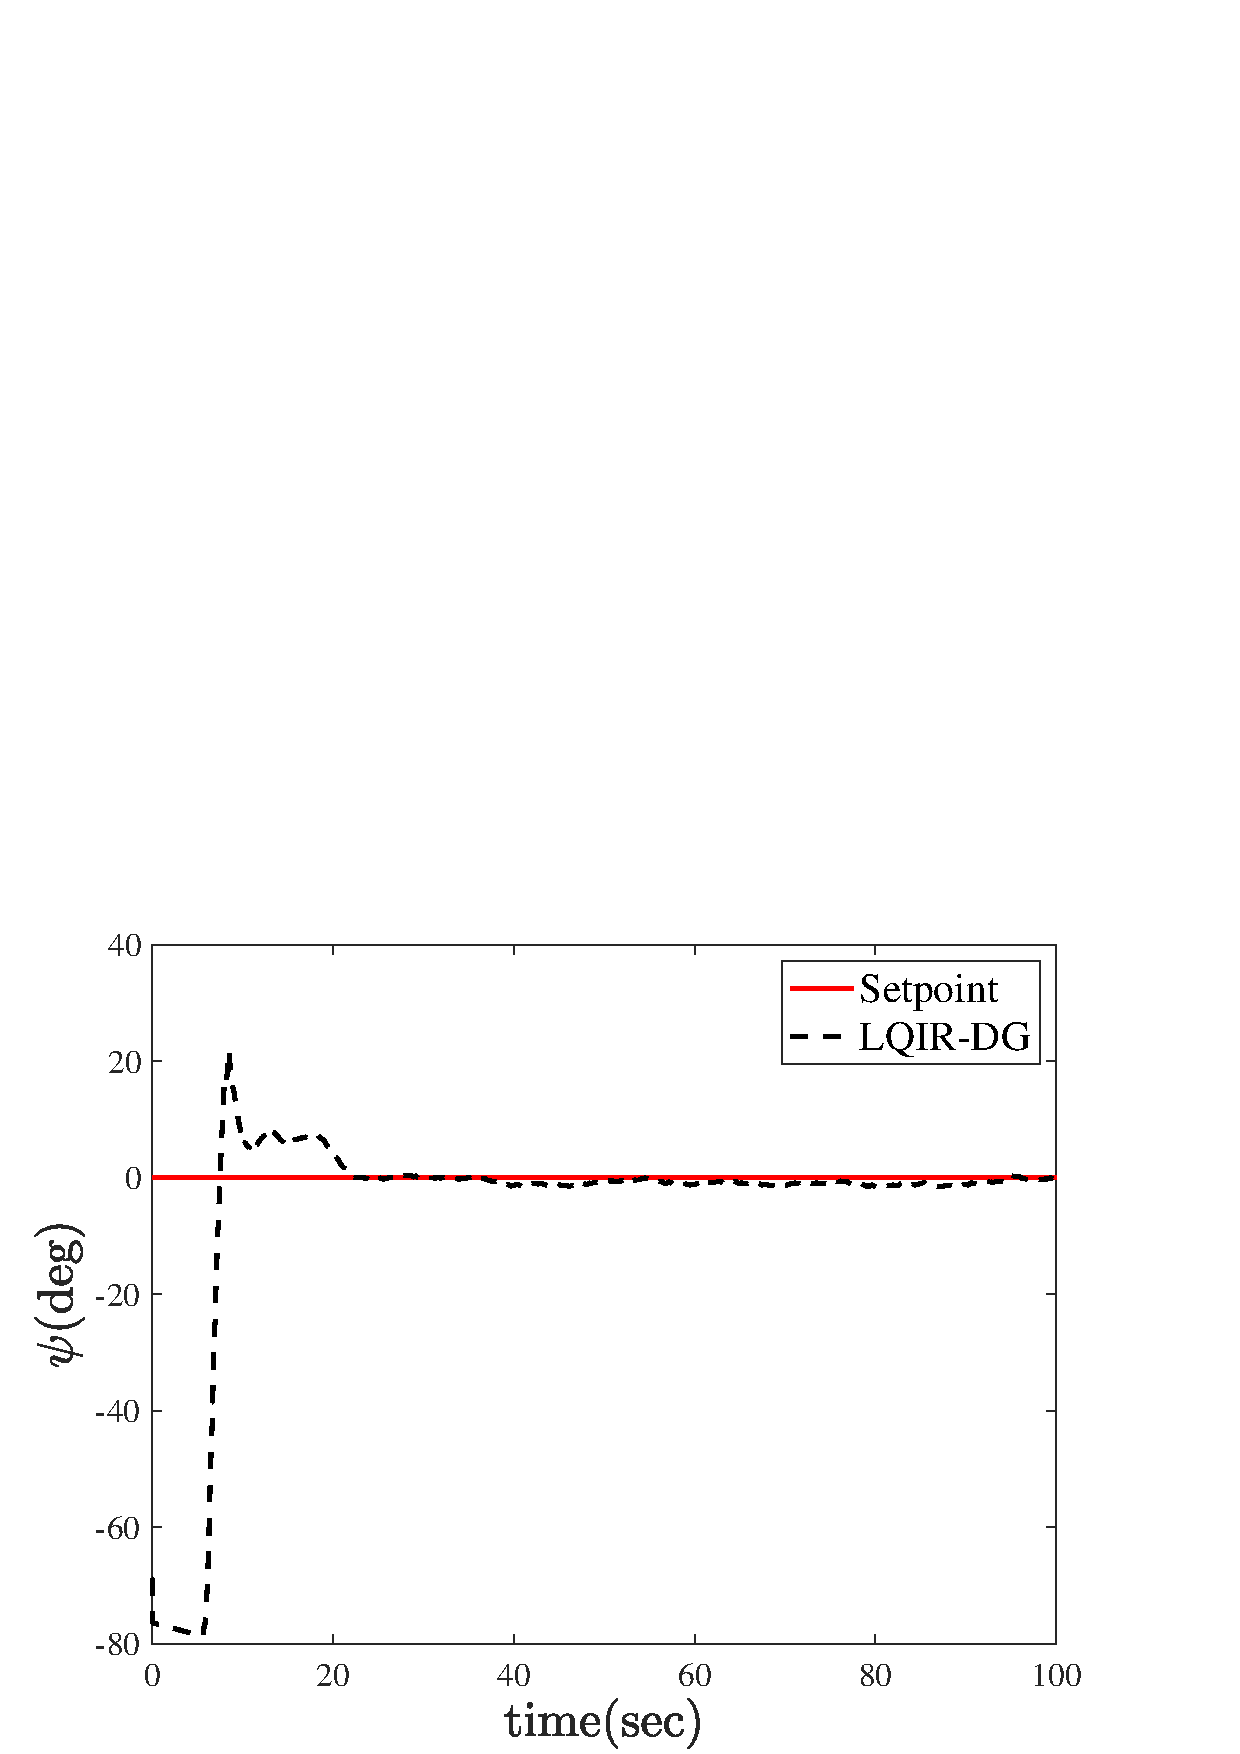
\includegraphics[width=12cm]{../Thesis/Figures/MIL/LQIDG/3DOF/lqidg_yaw.png}
			%		\caption{تغییرات زاویه یاو}
			%	\end{subfigure}
		%	\caption{عملکرد کنترل‌کننده LQIDG در کنترل زاویه رول، پیچ و یاد (تعقیب ورودی صفر)}
		%\end{figure}
		\begin{figure}[H]
			\centering
			\subfigure[تغییرات زاویه رول]{
				\centering
				\includegraphics[width=.48\linewidth]{../Thesis/Figures/MIL/LQIDG/3DOF/lqidg_roll_nn.png}
			}
			\subfigure[تغییرات زاویه پیچ]{
				\centering
				\includegraphics[width=.48\linewidth]{../Thesis/Figures/MIL/LQIDG/3DOF/lqidg_pitch_nn.png}
			}
			\subfigure[تغییرات زاویه یاو]{
				\centering
				\includegraphics[width=.48\linewidth]{../Thesis/Figures/MIL/LQIDG/3DOF/lqidg_yaw_nn.png}
			}
			\caption{عملکرد کنترل‌کننده \lr{LQIDG} در کنترل وضعیت (تعقیب ورودی صفر)}
			\label{lqidg_roll_pitch_yaw_fig_simulation_ll}
		\end{figure}
	 همانطور که از شکل
		\ref{lqidg_roll_pitch_yaw_fig_simulation_ll}
		مشخص است، زمان نشست برای کانال‌های مختلف حداکثر پنج ثانیه است. و خطای ماندگار وجود ندارد. در ادامه فرمان کنترلی موتورها آورده شده‌است.
		
		\begin{figure}[H]
			\centering
			\subfigure[موتور شماره یک]{
				\centering
				\includegraphics[width=.45\linewidth]{../Thesis/Figures/MIL/LQIDG/3DOF/lqidg_roll_pitch_Omega_1_nn.png}
			}
			\subfigure[موتور شماره دو]{
				\centering
				\includegraphics[width=.45\linewidth]{../Thesis/Figures/MIL/LQIDG/3DOF/lqidg_roll_pitch_Omega_2_nn.png}
			}
			\subfigure[موتور شماره سه]{
				\centering
				\includegraphics[width=.45\linewidth]{../Thesis/Figures/MIL/LQIDG/3DOF/lqidg_roll_pitch_Omega_3_nn.png}
			}
			\subfigure[موتور شماره چهار]{
				\centering
				\includegraphics[width=.45\linewidth]{../Thesis/Figures/MIL/LQIDG/3DOF/lqidg_roll_pitch_Omega_4_nn.png}
			}
			\caption{فرمان کنترلی موتورها در کنترل وضعیت (تعقیب ورودی صفر)}
		\end{figure}
		
		
%	\begin{equation}
%		\boldsymbol{K_{a_{1_{roll}}}} = \begin{bmatrix}
%			1720.86 & 80.29 & 187.71 & -8.57 \\
%			80.29 & 20.44 & 8.11 & 0.53 \\
%			187.77 & 8.11 & 686.56 & -0.02 \\
%			-8.57 & 0.53 & -0.02 & 9.93 \\
%		\end{bmatrix}, \boldsymbol{K_{a_{1_{pitch}}}} \begin{bmatrix}
%			243.90 & 25.01 & 80.29 & -9.50 \\
%			25.01 & 7.41 & 7.33 & 0 \\
%			80.29 & 7.33 & 239.14 & 0 \\
%			-9.50 & 0 & 0 & 9.50 \\
%		\end{bmatrix}
%	\end{equation}
	در نهایت فرمان کنترلی بهینه بازیکن اول از رابطه
	(\ref{LQIDG_u})
	به‌صورت زیر به دست می‌آید.
	\begin{equation}
		\begin{split}
			u_{1_{roll}} &= -\begin{bmatrix}
				79.7522 &20.4432 &8.1058 &0.5344 
			\end{bmatrix} \boldsymbol{x_{a_{roll}}} \\
			u_{1_{pitch}} &= -\begin{bmatrix}
				25.0112 &7.40730 &7.3280 &0.0010
			\end{bmatrix} \boldsymbol{x_{a_{pitch}}}
		\end{split}
	\end{equation}
	%\begin{figure}[H]
	%	\centering
	%	\begin{subfigure}
		%		\centering
		%		\includegraphics[width=12cm]{../Thesis/Figures/MIL/LQIDG/Roll_Pitch/lqidg_roll.png}
		%		\caption{تغییرات زاویه رول}
		%	\end{subfigure}%
	%	\begin{subfigure}
		%		\centering
		%		\includegraphics[width=12cm]{../Thesis/Figures/MIL/LQIDG/Roll_Pitch/lqidg_pitch.png}
		%		\caption{تغییرات زاویه پیچ}
		%	\end{subfigure}
	%	
	%\end{figure}
	\begin{figure}[H]
		\centering
		\subfigure[تغییرات زاویه رول]{
			\centering
			\includegraphics[width=.48\linewidth]{../Thesis/Figures/MIL/LQIDG/Roll_Pitch/lqidg_roll_nn.png}
		}
		\subfigure[تغییرات زاویه پیچ]{
			\centering
			\includegraphics[width=.48\linewidth]{../Thesis/Figures/MIL/LQIDG/Roll_Pitch/lqidg_pitch_nn.png}
		}
		\caption{عملکرد کنترل‌کننده \lr{LQIDG} در کنترل زاویه رول و پیچ (تعقیب ورودی صفر)}
		\label{lqidg_roll_pitch_fig_simulation}
	\end{figure}
	
	
	
	\begin{figure}[H]
		\centering
		\subfigure[موتور شماره یک]{
			\centering
			\includegraphics[width=.45\linewidth]{../Thesis/Figures/MIL/LQIDG/Roll_Pitch/lqidg_roll_pitch_Omega_1_nn.png}
		}
		\subfigure[موتور شماره دو]{
			\centering
			\includegraphics[width=.45\linewidth]{../Thesis/Figures/MIL/LQIDG/Roll_Pitch/lqidg_roll_pitch_Omega_2_nn.png}
		}
		\subfigure[موتور شماره سه]{
			\centering
			\includegraphics[width=.45\linewidth]{../Thesis/Figures/MIL/LQIDG/Roll_Pitch/lqidg_roll_pitch_Omega_3_nn.png}
		}
		\subfigure[موتور شماره چهار]{
			\centering
			\includegraphics[width=.45\linewidth]{../Thesis/Figures/MIL/LQIDG/Roll_Pitch/lqidg_roll_pitch_Omega_4_nn.png}
		}
		\caption{فرمان کنترلی موتورها در کنترل زاویه رول و پیچ (تعقیب ورودی صفر)}
	\end{figure}
 همانطور که از شکل
	\ref{lqidg_roll_pitch_fig_simulation}
	مشخص است، زمان نشست در برای هر دو کانال رول و پیچ حدود یک ثانیه است و خطای ماندگار وجود ندارد.
	
	
	
	
	
	
	
	\section{پیاده‌سازی کنترل‌کننده روی استند سه درجه آزادی چهارپره}
	%\ref{openloop_game}
	%و
	%\ref{closedloop_game}
	%کنترل‌کننده خطی مبتنی بر بازی دیفرانسیلی در حالت حلقه‌باز و حلقه‌بسته معرفی شد.
	
	% در بخش
	%\ref{roll_lqr_section_simulation}
	%ابتدا کانال رول استند چهارپره در حضور کنترل‌کننده \lr{LQR} و در ادامه در حضور کنترل‌کننده‌های \lr{LQDG} و \lr{LQIDG} شبیه‌سازی شد. سپس، کانال‌های رول-پیچ و رول-پیچ-یاو در بخش های
	%\ref{roll_lqr_section_simulation}
	%و
	%\ref{roll_pitch_lqidg_section_simulation_label}
	%%\ref{roll_pitch_lqidg_section_simulation}
	%در حضور کنترل‌کننده  \lr{LQIDG} شبیه‌سازی شدند. 
	%%\ref{roll_pitch_yaw_lqidg_section}
	%در این فصل به پیاده سازی کنترل‌کننده روی استند سه درجه آزادی چهارپره پرداخته شده‌است. در بخش 
	%\ref{roll_lqr_section}
	%به پیاده‌سازی کنترل‌کننده روی کانال پیچ پرداخته شده‌است. سپس، در بخش‌های 
	%\ref{roll_pitch_lqidg_section}
	%و
	%\ref{3DOF_lqidg_section}
	%به پیاده‌سازی کنترل‌کننده روی کانال‌های رول-پیچ و رول-پیچ-یاو پرداخته شده‌است. 
	
	\subsection{نتایج کنترل کانال پیچ}\label{roll_lqr_section}
	%در بخش
	%\ref{roll_lqr_section_simulation}
	%شبیه‌سازی تک کانال استند چهارپره در حضور کنترل‌کننده \lr{LQR} انجام شد. در این بخش به پیاده‌سازی کنترل‌کننده \lr{LQR} برای کانال پیچ استند سه درجه آزادی پرداخته می‌شود. 
	در پیاده‌سازی از ضرایب وزنی بهینه به دست آمده در قسمت شبیه‌سازی استفاده شده‌است.
	\begin{figure}[H]
		\includegraphics[width=.48\linewidth]{../Thesis/Figures/Calibration/LQR/Pitch/lqr_pitch.png}
		\centering
		\caption{عملكرد کنترل‌کننده \lr{LQR} در کنترل زاويه پیچ (تعقیب ورودی صفر)}
	\end{figure}
	%
	%\begin{figure}[H]
	%	[width=12cm]
	%	\centering
	%	\begin{subfigure}
		%		\centering
		%		\includegraphics[width=12cm]{../Thesis/Figures/Calibration/LQR/Pitch/lqr_pitch_Omega_1.png}
		%		\caption{موتور شماره یک}
		%	\end{subfigure}
	%	\begin{subfigure}
		%		\centering
		%		\includegraphics[width=12cm]{../Thesis/Figures/Calibration/LQR/Pitch/lqr_pitch_Omega_3.png}
		%		\caption{موتور شماره سه}
		%	\end{subfigure}
	%	\caption{فرمان کنترل‌کننده موتور سه و چهار در کنترل زاویه رول و پیچ (تعقیب ورودی صفر)}
	%\end{figure}
	\begin{figure}[H]
		\centering
		\subfigure[موتور شماره یک]{
			\centering
			\includegraphics[width=.45\linewidth]{../Thesis/Figures/Calibration/LQR/Pitch/lqr_pitch_Omega_1.png}
		}
		\subfigure[موتور شماره سه]{
			\centering
			\includegraphics[width=.45\linewidth]{../Thesis/Figures/Calibration/LQR/Pitch/lqr_pitch_Omega_3.png}
		}
		\caption{فرمان کنترلی موتورهای یک و سه در کنترل زاویه پیچ (تعقیب ورودی صفر)}
	\end{figure}
	%بر اساس خروجی شبیه‌سازی (شکل
	%\ref{lqr_roll_fig})
	%،کانال رول در حضور کنترل‌کننده \lr{LQR} در حدود پنج ثانیه به تعادل می‌رسد اما دارای خطای ماندگار است. 
	
	%\section{پیاده‌سازی کنترل‌کننده \lr{LQDG} بر رویه کانال پیچ}\label{roll_LQDG_section}
	%در بخش
	%\ref{roll_LQDG_section_simulation}
	%شبیه‌سازی تک کانال استند چهارپره در حضور کنترل‌کننده \lr{LQDG} انجام شد.
	کانال پیچ استند سه درجه آزادی در حضور کنترل‌کننده \lr{LQR} نوسانی و دارای خطای ماندگار است.
	در ادامه به پیاده‌سازی کنترل‌کننده \lr{LQDG} بر رویه کانال پیچ استند سه درجه آزادی پرداخته می‌شود.
	در پیاده‌سازی از ضرایب وزنی بهینه به دست آمده در قسمت شبیه‌سازی استفاده شده‌است.
	\begin{figure}[H]
		\includegraphics[width=.48\linewidth]{../Thesis/Figures/Calibration/LQDG/Pitch/lqdg_pitch.png}
		\centering
		\caption{عملكرد کنترل‌کننده \lr{LQDG} در کنترل زاويه پیچ (تعقیب ورودی صفر)}
	\end{figure}
	
	\begin{figure}[H]
		\centering
		\subfigure[موتور شماره یک]{
			\centering
			\includegraphics[width=.45\linewidth]{../Thesis/Figures/Calibration/LQDG/Pitch/lqdg_pitch_Omega_1.png}
		}
		\subfigure[موتور شماره سه]{
			\centering
			\includegraphics[width=.45\linewidth]{../Thesis/Figures/Calibration/LQDG/Pitch/lqdg_pitch_Omega_3.png}
		}
		\caption{فرمان کنترلی موتورهای یک و سه در کنترل زاویه پیچ (تعقیب ورودی صفر)}
	\end{figure}



%\ref{lqdg_roll_fig})
%،کانال رول در حضور کنترل‌کننده \lr{LQDG} در کمتر از پنج ثانیه به تعادل می‌رسد اما دارای خطای ماندگار است ولی خطای مانگار آن نسبت به کنترل‌کننده بخش
%\ref{roll_lqr_section}
%کمتر است. به دلیل خطای ماندگار، در بخش
%%LQIDG
%انتگرال‌گیر به کنترل‌کننده اضافه می‌شود تا خطای مانگار استند را کم کند.


%\section{پیاده‌سازی کنترل‌کننده \lr{LQIDG} بر رویه کانال پیچ}\label{roll_lqidg_section}
%در بخش
%\ref{roll_lqidg_section_simulation}
%شبیه‌سازی تک کانال استند چهارپره در حضور کنترل‌کننده \lr{LQIDG} انجام شد. 
کانال پیچ استند سه درجه آزادی در حضور کنترل‌کننده \lr{LQDG} نوسانی و دارای خطای ماندگار است.
در ادامه به پیاده‌سازی کنترل‌کننده \lr{LQIDG} بر رویه کانال پیچ استند سه درجه آزادی پرداخته می‌شود.
در پیاده‌سازی از ضرایب وزنی بهینه به دست آمده در قسمت شبیه‌سازی استفاده شده‌است.
\begin{figure}[H]
	\includegraphics[width=.48\linewidth]{../Thesis/Figures/Calibration/LQIDG/Pitch/lqidg_pitch.png}
	\centering
	\caption{عملكرد کنترل‌کننده  LQIDG در کنترل زاويه پیچ (تعقیب ورودی صفر)}
\end{figure}

%\begin{figure}
%	[width=12cm]
%	\centering
%	\begin{subfigure}
	%		\centering
	%		\includegraphics[width=12cm]{../Thesis/Figures/Calibration/LQIDG/Pitch/lqidg_Omega_1.png}
	%		\caption{موتور شماره یک}
	%	\end{subfigure}
%	\begin{subfigure}
	%		\centering
	%		\includegraphics[width=12cm]{../Thesis/Figures/Calibration/LQIDG/Pitch/lqidg_Omega_3.png}
	%		\caption{موتور شماره سه}
	%	\end{subfigure}
%	\caption{فرمان کنترل‌کننده موتور سه و چهار در کنترل زاویه رول و پیچ (تعقیب ورودی صفر)}
%\end{figure}

\begin{figure}[H]
	\centering
	\subfigure[موتور شماره یک]{
		\centering
		\includegraphics[width=.45\linewidth]{../Thesis/Figures/Calibration/LQIDG/Pitch/lqidg_Omega_1.png}
	}
	\subfigure[موتور شماره سه]{
		\centering
		\includegraphics[width=.45\linewidth]{../Thesis/Figures/Calibration/LQIDG/Pitch/lqidg_Omega_3.png}
	}
	
	\caption{فرمان کنترلی موتورهای یک و سه در کنترل زاویه پیچ (تعقیب ورودی صفر)}
\end{figure}
کانال پیچ استند سه درجه آزادی در حضور کنترل‌کننده \lr{LQIDG} عملکرد خوبی از خود نشان می‌دهد و به علت وجود انتگرال‌گیر خطای ماندگار ندارد.



%\section{پیاده‌سازی کنترل‌کننده \lr{LQIDG} بر رویه کانال پیچ}\label{roll_lqidg_section}
%در بخش
%\ref{roll_lqidg_section_simulation}
%شبیه‌سازی تک کانال استند چهارپره در حضور کنترل‌کننده \lr{LQIDG} انجام شد. 
کانال پیچ استند سه درجه آزادی در حضور کنترل‌کننده \lr{LQDG} نوسانی و دارای خطای ماندگار است.
در ادامه به پیاده‌سازی کنترل‌کننده \lr{LQIDG} بر رویه کانال پیچ استند سه درجه آزادی پرداخته می‌شود.
در پیاده‌سازی از ضرایب وزنی بهینه به دست آمده در قسمت شبیه‌سازی استفاده شده‌است.
\begin{figure}[H]
	\includegraphics[width=.48\linewidth]{../Thesis/Figures/Calibration/LQIDG/Pitch/lqidg_pitch.png}
	\centering
	\caption{عملكرد کنترل‌کننده  LQIDG در کنترل زاويه پیچ (تعقیب ورودی صفر)}
\end{figure}

%\begin{figure}
%	[width=12cm]
%	\centering
%	\begin{subfigure}
	%		\centering
	%		\includegraphics[width=12cm]{../Thesis/Figures/Calibration/LQIDG/Pitch/lqidg_Omega_1.png}
	%		\caption{موتور شماره یک}
	%	\end{subfigure}
%	\begin{subfigure}
	%		\centering
	%		\includegraphics[width=12cm]{../Thesis/Figures/Calibration/LQIDG/Pitch/lqidg_Omega_3.png}
	%		\caption{موتور شماره سه}
	%	\end{subfigure}
%	\caption{فرمان کنترل‌کننده موتور سه و چهار در کنترل زاویه رول و پیچ (تعقیب ورودی صفر)}
%\end{figure}

\begin{figure}[H]
	\centering
	\subfigure[موتور شماره یک]{
		\centering
		\includegraphics[width=.45\linewidth]{../Thesis/Figures/Calibration/LQIDG/Pitch/lqidg_Omega_1.png}
	}
	\subfigure[موتور شماره سه]{
		\centering
		\includegraphics[width=.45\linewidth]{../Thesis/Figures/Calibration/LQIDG/Pitch/lqidg_Omega_3.png}
	}
	
	\caption{فرمان کنترلی موتورهای یک و سه در کنترل زاویه پیچ (تعقیب ورودی صفر)}
\end{figure}
کانال پیچ استند سه درجه آزادی در حضور کنترل‌کننده \lr{LQIDG} عملکرد خوبی از خود نشان می‌دهد و به علت وجود انتگرال‌گیر خطای ماندگار ندارد.



%بر اساس خروجی شبیه‌سازی (شکل
%\ref{lqidg_roll_fig})
%،کانال رول در حضور کنترل‌کننده LQIDG در حدود پنج ثانیه به تعادل می‌رسد و خطای ماندگار آن در حدود صفر است.


\subsection{نتایج کنترل کانال رول-پیچ}\label{roll_pitch_lqidg_section}
%در بخش
%\ref{roll_pitch_lqidg_section_simulation}
%شبیه‌سازی کانال رول-پیچ استند چهارپره در حضور کنترل‌کننده \lr{LQIDG} انجام شد. 
در ادامه به پیاده‌سازی کنترل‌کننده \lr{LQIDG} روی کانال رول-پیچ استند سه درجه آزادی از شرایط اولیه
$\phi = 5^{\circ}$
و
$\theta = -60^{\circ}$
پرداخته شده‌است.
در پیاده‌سازی از ضرایب وزنی بهینه به دست آمده در قسمت شبیه‌سازی استفاده شده‌است.

\begin{figure}[H]
	\centering
	\subfigure[تغییرات زاویه رول]{
		\centering
		\includegraphics[width=.48\linewidth]{../Thesis/Figures/Calibration/LQIDG/Roll_Pitch/lqidg_roll.png}
	}
	\subfigure[تغییرات زاویه پیچ]{
		\centering
		\includegraphics[width=.48\linewidth]{../Thesis/Figures/Calibration/LQIDG/Roll_Pitch/lqidg_pitch.png}
	}
	\caption{عملکرد کنترل‌کننده \lr{LQIDG} در کنترل زاویه رول و پیچ (تعقیب ورودی صفر)}
\end{figure}

\begin{figure}[H]
	\centering
	\subfigure[موتور شماره یک]{
		\centering
		\includegraphics[width=.45\linewidth]{../Thesis/Figures/Calibration/LQIDG/Roll_Pitch/lqidg_Omega_1.png}
	}
	\subfigure[موتور شماره دو]{
		\centering
		\includegraphics[width=.45\linewidth]{../Thesis/Figures/Calibration/LQIDG/Roll_Pitch/lqidg_Omega_2.png}
	}
	\subfigure[موتور شماره سه]{
		\centering
		\includegraphics[width=.45\linewidth]{../Thesis/Figures/Calibration/LQIDG/Roll_Pitch/lqidg_Omega_3.png}
	}
	\subfigure[موتور شماره چهار]{
		\centering
		\includegraphics[width=.45\linewidth]{../Thesis/Figures/Calibration/LQIDG/Roll_Pitch/lqidg_Omega_4.png}
	}
	\caption{فرمان کنترلی موتورها در کنترل زاویه رول و پیچ (تعقیب ورودی صفر)}
\end{figure}


\section{نتایج کنترل وضعیت}\label{3DOF_lqidg_section}
فرم خطی فضای حالت کانال‌های چهارپره محاسبه شده‌است. در بخش‌های
در ادامه به پیاده‌سازی کنترل‌کننده برای وضعیت استند سه درجه آزادی انجام شده‌است.
%\subsection{پیاده‌سازی کنترل‌کننده \lr{LQIDG} بر رویه استند به‌صورت سه کانال تک ورودی}
%\subsection{پیاده‌سازی کنترل‌کننده به‌صورت چهار ورودی}\label{lqidg_mimo}
%
%
%\begin{figure}[H]
%	\centering
%	\subfigure[تغییرات زاویه رول]{
	%		\centering
	%		\includegraphics[width=.48\linewidth]{../Thesis/Figures/Calibration/LQIDG/MIMO/lqidg_roll.png}
	%	}
%	\subfigure[تغییرات زاویه پیچ]{
	%		\centering
	%		\includegraphics[width=.48\linewidth]{../Thesis/Figures/Calibration/LQIDG/MIMO/lqidg_pitch.png}
	%	}
%	\subfigure[تغییرات زاویه یاو]{
	%		\centering
	%		\includegraphics[width=.48\linewidth]{../Thesis/Figures/Calibration/LQIDG/MIMO/lqidg_yaw.png}
	%	}
%	\caption{عملکرد کنترل‌کننده \lr{LQIDG} در کنترل وضعیت (تعقیب ورودی صفر)}
%\end{figure}
%
%
%
%\begin{figure}[H]
%	\centering
%	\subfigure[موتور شماره یک]{
	%		\centering
	%		\includegraphics[width=.45\linewidth]{../Thesis/Figures/Calibration/LQIDG/MIMO/lqidg_Omega_1.png}
	%	}
%	\subfigure[موتور شماره دو]{
	%		\centering
	%		\includegraphics[width=.45\linewidth]{../Thesis/Figures/Calibration/LQIDG/MIMO/lqidg_Omega_2.png}
	%	}
%	\subfigure[موتور شماره سه]{
	%		\centering
	%		\includegraphics[width=.45\linewidth]{../Thesis/Figures/Calibration/LQIDG/MIMO/lqidg_Omega_3.png}
	%	}
%	\subfigure[موتور شماره چهار]{
	%		\centering
	%		\includegraphics[width=.45\linewidth]{../Thesis/Figures/Calibration/LQIDG/MIMO/lqidg_Omega_4.png}
	%	}
%	\caption{فرمان کنترلی موتورها در کنترل وضعیت (تعقیب ورودی صفر)}
%\end{figure}
%\subsection{پیاده‌سازی کنترل‌کننده به‌صورت سه کانال تک ورودی}\label{lqidg_siso}
در بخش
\ref{roll_pitch_yaw_lqidg_section_ll}
شبیه‌سازی سه درجه آزادی استند چهارپره در حضور کنترل‌کننده \lr{LQIDG} انجام شد. در این بخش به پیاده‌سازی کنترل‌کننده \lr{LQIDG} روی استند سه درجه آزادی از شرایط اولیه
$\phi = 5^{\circ}$،
$\theta = 60^{\circ}$
و
$\psi = 100^{\circ}$
پرداخته شده‌است.
در پیاده‌سازی از ضرایب وزنی بهینه به دست آمده در قسمت شبیه‌سازی استفاده شده‌است.


\begin{figure}[H]
	\centering
	\subfigure[تغییرات زاویه رول]{
		\centering
		\includegraphics[width=.48\linewidth]{../Thesis/Figures/Calibration/LQIDG/3DOF/lqidg_roll.png}
	}
	\subfigure[تغییرات زاویه پیچ]{
		\centering
		\includegraphics[width=.48\linewidth]{../Thesis/Figures/Calibration/LQIDG/3DOF/lqidg_pitch.png}
	}
	\subfigure[تغییرات زاویه یاو]{
		\centering
		\includegraphics[width=.48\linewidth]{../Thesis/Figures/Calibration/LQIDG/3DOF/lqidg_yaw.png}
	}
	\caption{عملکرد کنترل‌کننده \lr{LQIDG} در کنترل وضعیت (تعقیب ورودی صفر)}
\end{figure}



\begin{figure}[H]
	\centering
	\subfigure[موتور شماره یک]{
		\centering
		\includegraphics[width=.45\linewidth]{../Thesis/Figures/Calibration/LQIDG/3DOF/lqidg_Omega_1.png}
	}
	\subfigure[موتور شماره دو]{
		\centering
		\includegraphics[width=.45\linewidth]{../Thesis/Figures/Calibration/LQIDG/3DOF/lqidg_Omega_2.png}
	}
	\subfigure[موتور شماره سه]{
		\centering
		\includegraphics[width=.45\linewidth]{../Thesis/Figures/Calibration/LQIDG/3DOF/lqidg_Omega_3.png}
	}
	\subfigure[موتور شماره چهار]{
		\centering
		\includegraphics[width=.45\linewidth]{../Thesis/Figures/Calibration/LQIDG/3DOF/lqidg_Omega_4.png}
	}
	\caption{فرمان کنترلی موتورها در کنترل وضعیت (تعقیب ورودی صفر)}
\end{figure}




%بر اساس خروجی شبیه‌سازی (شکل
%\ref{lqidg_roll_fig})
%،کانال رول در حضور کنترل‌کننده \lr{LQIDG} در حدود پنج ثانیه و کانال پیچ در حدود هشت ثانیه به تعادل می‌رسد و خطای ماندگار آن در حدود صفر است.










	
	
	%بر اساس خروجی شبیه‌سازی (ش
	
	
	%بر اساس خروجی شبیه‌سازی (شکل
	%\ref{lqidg_roll_fig})
	%،کانال رول در حضور کنترل‌کننده LQIDG در حدود پنج ثانیه به تعادل می‌رسد و خطای ماندگار آن در حدود صفر است.
	
	
	
	
	
	
	
	
	
	
	
%\section{قواعد نگارشی}
%
%شیوایی و رسایی نوشتار در گرو ساده‌نویسی است. تلاش شود در متن مقاله از جملات رسا، گویا، و کوتاه استفاده شود و از نوشتن جملات تودرتو پرهیز شود. به این جمله دقت کنید: «آهنگی که شما از فروشگاه
%\lr{iTune}
% دریافت می‌کنید توسط قالب
%\lr{DRM}
% اپل که یک قالب فایل 
% \lr{AAC}
%  انحصاری و محافظت شده است که اپل مجوز استفاده از آن را به هیچ کس نمی‌دهد، محافظت می‌شود». این جمله در واقع از سبک نگارش زبان انگلیسی پیروی می‌کند و به هیچ وجه برای جملات پارسی مناسب نیست. به راحتی می‌توان این جمله را به این صورت بازنویسی کرد: «آهنگی که شما از فروشگاه 
%\lr{iTune}
% دریافت می‌کنید توسط قالب
%\lr{DRM}
%   اپل محافظت می‌شود. این قالب یک قالب فایل
%\lr{AAC}
% انحصاری و محافظت شده است، و اپل مجوز استفاده از آن را به هیچ کس نمی‌دهد».
%
%جداسازی اجزای مختلف یک جمله نیز نقش زیادی در فهم آسان آن دارد. ویرگول می­تواند اجزای یک جمله را در جایی که نیاز به مکث هست، ازهم جدا کند؛ حال آن که نقطه ویرگول برای جداسازی دوجمله که با هم ارتباط معنایی دارند، بکار می­رود. نقطه نیز برای جدا کردن جملات مورد استفاده قرار می­گیرد. درکاربرد هلالین (پرانتز) باید توجه شود که عبارت داخل آن برای توضیحی است که از اجزای جمله محسوب نشده و درصورت حذف خللی به آن وارد نمی­شود. درمقابل، گیومه برای برجسته کردن جزیی از جمله بکار می­رود.
%
%تا جای ممکن از بکار بردن کلماتی مثل «می­باشد»، «گردید»، و «بوده باشد» پرهیز شود. به جای آن‌ها اغلب می‌توان از کلمات ساده و روان مثل «است» و «شد» استفاده کرد. بکارگیری کلمات دشوار و غیرمعمول تنها باعث پیچیده شدن جمله و دشوار شدن فهم آن می‌شود.
%
%برای کلمات فنی تا حد امکان از معادل‌های پارسی استفاده شود. بدون تردید کلمه «پردازش» زیباتر از «پروسس» است، و یا کلمه «ریزپردازنده» از «میکروپروسسور» مناسب‌تر است. در چنین مواقعی اگر احتمال می‌دهید خواننده با معادل پارسی آشنا نیست، از پانویس برای نوشتن معادل انگلیسی استفاده کنید. این کار را در اولین کاربرد معادل‌های پارسی انجام دهید. مثل گره راهنما
%\LTRfootnote{Anchor Node}.
%
%تا حد امکان از کلمات انگلیسی در جملات استفاده نکنید. مثلاٌ بجای نوشتن
%\lr{Microsoft}
% می­توانید بنویسید: «میکروسافت». اگر ناچار شدید در یک جمله از کلمات انگلیسی استفاده کنید، حتماً فاصله کافی بین آن‌ها و کلمات پارسی را رعایت کنید.
%
%\subsection{علامت‌گذاری}
%برای خوانایی بهتر مقاله باید سعی شود تا حد امکان علامت­گذاری متن مقاله بدرستی انجام شود. دقت کنید تمام علامت‌هایی مثل نقطه، ویرگول، نقطه ویرگول، دونقطه، و علامت سوال باید به کلمه قبل از خود چسبیده باشند، و از کلمه بعدی تنها به اندازه یک فضای خالی فاصله داشته باشند. علامت خط تیره باید به اندازه یک فضای خالی از کلمه قبل و بعد از خود فاصله داشته باشد؛ مگر این که کلمه قبلی یا بعدی یک عدد باشد، که در این صورت باید به آن بچسبد. بین کلماتی که جدا هستند باید یک فضای خالی فاصله باشد.
%\subsection{املا}
%درستی نوشتار بر پایه املای زبان پارسی ضروری است. در این بخش برخی از موارد اشتباه متداول را یادآوری می‌کنیم. می‌توانید اطلاعات دقیق‌تر را با مراجعه به کتاب­های نوشته شده در این زمینه پیدا کنید.
%
%در افعال حال و گذشته استمراری باید دقت شود که «می» از جزء بعدی فعل جدا نماند. برای این منظور می‌توانید از نیم‌فاصله استفاده کنید.
%
%در مورد «ها»ی جمع نیز دقت کنید که از کلمه جمع بسته شده جدا نوشته شود؛ مگر در کلمات تک هجایی مثل «آنها». برای جدانویسی نیز از فاصله متصل استفاده کنید. مثلاٌ «پردازنده ها» را بصورت «پردازنده‌­ها» بنویسید.
%
%جمع بستن کلمات پارسی یا لاتین با قواعد زبان عربی اشتباه است. بنابراین «پیشنهادات» و «اساتید» اشتباه و درست آنها «پیشنهادها» و «استادان» است.
%
%بهتر است همواره حرف اضافه «به» از کلمه بعدی خود جدا نوشته شود، مگر آن که این حرف جزء یک فعل یا صفت یا قید باشد؛ مانند: «بکار بستن»، «بجا» و «بندرت».
%
%در مورد کلمات حاوی همزه قواعدی وجود دارد که پرداختن به آنها دراین مقاله نمی­گنجد، اما برای نمونه به املای کلمات «مسأله»، «منشأ» و «رئیس» دقت کنید. همچنین، همزه در انتهای کلماتی که به الف ختم می­شوند، نوشته نمی­شود و درصورت اضافه شدن به کلمه بعدی، از «ی» استفاده می­شود: «اجرا شده»، و «اجرای برنامه».
%
%
%\subsection{شکل‌ها و جدول­ها}
%شکل‌ها و جدول­ها باید دارای عنوان باشند. عنوان شکل‌ها در زیر شکل و عنوان جدول­ها در بالای جدول قرار می‌گیرند. در صورتی که از شکل‌ها یا جدول­های سایر منابع استفاده می‌کنید، باید حتماً شماره آن مرجع را در عنوان شکل یا جدول ذکر کنید.
%
%در هنگام ارجاع به شکل یا جدول از شماره آن استفاده کنید و از بکار بردن عباراتی همچون «شکل زیر» پرهیز کنید. تمام جدول­ها و شکل‌ها باید در متن مورد ارجاع قرار گیرند. 
%
%
%\subsection{ فرمول‌ها و عبارات ریاضی}
%برای هر فرمول باید یک شماره در نظر گرفته شود. این شماره را در داخل یک جفت هلالین و بصورت راست‌چین قرار دهید.  در  
% \lr{\LaTeX}
%   شماره گذاری به صورت خودکار انجام می‌پذیرد. تمام متغیرها، پارامترها، و نمادهای یک عبارت ریاضی باید توضیح داده شوند. اگر قبل از نوشتن فرمول این کار انجام نشده است، باید بلافاصله پس از فرمول این توضیحات بیان شوند. مثال زیر را در نظر بگیرید.
%
%اگر 
%$\rho$
% بیانگر چگالی تخمینی باشد، خواهیم داشت:
%\begin{equation}
%\rho = \frac{m}{A},
%\end{equation}
%که درآن  $m$ جرم تخمینی و $A$ سطح آن است. 
%
%اگر در مقاله شما نمادهای ریاضی متنوعی مورد استفاده قرار می‌گیرد، حتما سعی کنید جدول نمادها در متن خود داشته باشید. مثل جدول 
%\ref{tab:symbols}.
%
%\begin{table}[t]
%\centering
%\caption{نمادهای مورد استفاده در  مقاله}
%\label{tab:symbols}
%\begin{tabular}{cp{6cm}}\hline
%نماد & توضیحات
%\\\hline
%$N$ &
%تعداد کل گره‌های شبکه
%\\
%$\mathbb{R}^{++}$ &
%مجموعه اعداد حقیقی مثبت بزرگتر از صفر
%\\
%$\rho_{t}$ &
%چگالی شبکه در لحظه $t$
%\\
%$\mathrm{Pr}[A]$ &
%احتمال رخداد رویداد $A$
%\\
%\hline
%\end{tabular}
%\end{table}
%
%
%
%\section{نکاتی در مورد نوشتن مقاله با \lr{\LaTeX}}
%نویسندگانی که با محیط
%\lr{\LaTeX}
% و نحوه کار با آن آشنایی ندارند می‌توانند به سایت
%\url{www.parsilatex.com}
%مراجعه کنند. مطالب مفید بسیاری در این زمینه در سایت مذکور قرار داده شده است. 
%برای پردازش این فایل کافیست یک توزیع تِک به مانند
% \lr{TeXLive}
% را نصب داشته باشید.
% 
%لازم به ذکر است که تمامی عبارت‌ها و کلمات انگلیسی در فایل
% \lr{\LaTeX}
%  باید درون دستور
% \lr{lr}
%  قرار گیرند. مثلا:
%\lr{Support vector}
% و یا
%\lr{Machine Learning}.
%دقت کنید که تمامی کلمات و عبارت‌های اختصاری می‌بایست در اولین فراخوانی به صورت باز شده ارایه شود. به عنوان مثال در اولین مکانی که شما از کلمه اختصاری 
%\lr{SVM}
% استفاده می‌کنید باید آن را به صورت 
%\lr{SVM (support vector machine)}
%بنویسید. به صورت معمول تمامی حروف حالت بازشده باید با حرف کوچک نوشته شود.
%
%ترجیحا توصیه می‌شود که نویسندگان از قراردادن پاورقی در مقاله پرهیز کنند، اما در صورت نیاز شما می‌توانید با دستور 
%\lr{footnote}
% پاورقی فارسی و با دستور
%\lr{LTRfootnote}
% پاورقی انگلیسی قرار دهید. مثل: در این روش
%\footnote{در واقع منظور ما ...}
% و یا حسگر
%\LTRfootnote{Sensor}.
% دقت کنید که همه پاورقی‌ها در انتهای متن در بخشی به نام پانویس چاپ خواهند شد و نه در همان صفحه.
%
%در صورتی که می‌خواهید بر روی یک کلمه و یا عبارت در یک متن تاکید کنید، لطفا از دستور
% \lr{emph} 
% استفاده کنید، مثل: کار اصلی ما در این مقاله ارایه یک روش
%\emph{داده‌کاوی}
%است. تقریبا تمامی بسته‌های مورد نیاز برای نوشتن یک مقاله در استایل 
%\lr{\LaTeX}
% تهیه شده قرار داده شده است. اما در صورت نیاز به یک بسته معین لطفا استایل قرار داده شده را تغییر دهید و قبل از فراخوانی بسته‌های
%\lr{hyperref}
% و بسته 
%\lr{\XePersian} 
% بسته خود را وارد کنید. در هنگام آپلود مقاله نیز کل فایل‌های 
%\lr{\LaTeX} 
% -- به جز فایلهای فونت-- باید به صورت
%\lr{zip} 
% شده در سایت مورد نظر قرار داده شود. محتویات فایل با پسوند
%\lr{zip}
% باید شامل خروجی 
%\lr{pdf}،
% تمامی تصاویر، فایل اصلی 
%\lr{tex}، 
% فایل با پسوند
%\lr{bib}
% و هر فایل دیگر مورد نیاز باشد.
%
%برای نوشتن فرمول یک خطی در
% \lr{\LaTeX}
%  به سادگی می‌توانید از محیط 
%  \lr{equation}
%   استفاده کنید. مثل:
%\begin{equation}
%A = B^2 + \frac{\gamma}{4}.
%\label{eq:dols}
%\end{equation}
%روابط می‌بایست در صورت نیاز حتما شماره‌گذاری شوند. برای عدم شماره‌گذاری می‌توانید از محیط 
%\lr{equation*}
% بهره بگیرید.مثل:
%\begin{equation*}
%A = \frac{\gamma}{\zeta}, \quad\quad \gamma\in\mathbb{R}^{++}.
%\end{equation*}
%برای روابط چندخطی از محیط
% \lr{align}
%  استفاده کنید. مثل:
%\begin{align}
%A =& B^c+\alpha \nonumber\\
%R =& A + T.
%\label{eq:sams}
%\end{align}
%و یا به عنوان مثال دیگر:
%\begin{align}
%\mathrm{H}(\lambda_{g}|\lambda_{g}+\lambda_{d})  =& \frac{1}{N}\sum_{i=1}^{N}\log_{2}(N-i+1) \nonumber\\
%&+  \frac{1}{N}\sum_{i=1}^{N}\frac{\sum_{j=i}^{N}\log_{2}(\Upsilon_{N}-\Upsilon_{N-j})}{N-i+1}, \nonumber\\
%=& \sum_{i=1}^{N}\frac{\sum_{j=i}^{N}\log_{2}(\Upsilon_{N}-\Upsilon_{N-j})}{N(N-i+1)}.
%\label{eq:conditionalentorpyresult}
%\end{align}
%
%
%برای ارجاع به روابط و فرمول‌ها نیاز نیست بنویسید مثلا فرمول شماره ..، فقط کافی است که برچسب فرمول را با دستور
% \lr{eqref}
%  فراخوانی کنید. در این صورت نیازی به قرار دادن پرانتز نیست و
%   \lr{\LaTeX}
%    به صورت خودکار پرانتزها را می‌گذارد. مثلا با قرار دادن
%     \eqref{eq:sams}
%      در 
%      \eqref{eq:dols}
%       خواهیم داشت ... 
%
%سعی کنید مطالب خود را به صورت منظم در قالب تعدادی تعریف، قضیه، لم و گزاره بیاورید. تمامی این محیط‌های در استایل آماده شده تعریف شده است و براحتی قابل استفاده است.
%\begin{definition}[حالت پایدار]
%حالتی را پایدار گوییم که در آن تغییر آمارگان پارامترهای صف برابر صفر باشد. اگر $\varpi$ را یک پارامتر صف در نظر بگیریم، خواهیم داشت.
%\begin{equation}
%\frac{\mathrm{d}\varpi(t)}{\mathrm{d}t}=0
%\end{equation}
%\end{definition}
%
%\begin{theorem}[پایستگی جریان]
%در صورتی که سامانه مورد بررسی ارگودیک و در پایدار باشد، آن‌گاه نرخ ورود بسته به سامانه همواره برابر با نرخ خروج آن خواهد بود. 
%\label{theorem:jddkssskaa}
%\end{theorem}
%\begin{theorem}
%قرار دادن نام برای قضیه به مانند قضیه قبل که نامش پایستگی جریان بود اختیاری است.
%\label{theorem:jdtysssaa}
%\end{theorem}
%\begin{proof}
%سعی کنید اگر قضیه برای مرجع دیگری است اثبات آن را در مقاله نیاورید و فقط به مرجع مذکور ارجاع دهید. اگر اثبات در روند مقاله اهمیت دارد آن را درون متن مقاله بیاورید. اما اگر در روند کلی تاثیری ندارد اثبات را به قسمت پیوست‌ها ببرید. 
%\end{proof}
%\begin{corollary}
%در یک صف نرخ ورود با خروج برابر است.
%\end{corollary}
%\begin{corollary}
%در یک سامانه نرخ ورود برابر است با تعداد بسته‌ها ....
%\end{corollary}
%\begin{lemma}
%   اگر $N_t$ نشان‌دهنده تعداد بسته رسیده تا زمان $t$ به .......
%\begin{equation}
%P(t_{i}>t)=P(N(t)<i)\Longrightarrow P(t_{i}<t)=1-
%\end{equation}
%
%\end{lemma}%%
%\begin{proof}
%برای اثبات به مرجع .... برای اثبات قضایا از محیط 
%\lr{proof}
% استفاده کنید.
%\end{proof}
%
%\begin{principle}[عدم قطعیت]
%برطبق اصل عدم قطعیت هر ذره ....
%\end{principle}
%
%توصیه می‌شود که نویسندگان برای نمادهای ریاضیاتی سعی کنند از نمادهای ساده و استاندارد استفاده کنند. به عنوان مثال مجموعه اعداد حقیقی را بهتر است به جای
% $R$ با $\mathbb{R}$
%  نشان داد. تمامی عملگرهای ریاضیاتی به مانند عملگر امیدریاضی، آنتروپی، احتمال رخداد یک رویداد باید به صورت غیرایتالیک نوشته شود، مثل:
%$\mathrm{E}[..]$, $\mathrm{Pr}[..]$, $\mathrm{H}[..]$ و ... . 
%
%نویسندگان می‌بایست حتما و حتما نمادها و روابط ریاضی موجود در متن را در حالت 
%\lr{math mode}
% بنویسند و نه در حالت متنی. به عنوان مثال به جای 
% \lr{A+B}
%  که به صورت متنی است، بهتر است بنویسید $A+B$.
%\section{نتیجه گیری}
%در این بخش نویسندگان باید به صورت خلاصه کل روندی که در مقاله پیموده شده است را توضیح دهند. در ضمن نویسندگان می‌توانند در این بخش ایده‌های جدید برای توسعه هرچه بیشتر و بهتر مقاله خود را مطرح کنند.
%
%\section*{سپاس‌گزاری}
%بخش سپاس‌گزاری در صورت نیاز بصورت کوتاه و در یک بند آماده شود. بخش سپاسگزاری دارای شماره نیست. 
%
%\section*{پیوست‌ها}
%بخش پیوست‌ها یک بخش اختیاری است و شماره‌گذاری  نمی‌شود. موضوع‌های مرتبط با مقاله که در یکی از گروه‌های زیر قرار گیرند، می‌توانند در بخش ضمایم آورده شوند.
%\begin{itemize}
%\item
%اثبات ریاضی فرمول‌ها یا الگوریتم‌ها.
%\item
%داده‌ها و اطلاعات مربوط به مطالعه موردی.
%\item
%نتایج کار دیگر محققان و داده‌های مربوط به مقایسه آن‌ها.
%\item
%سایر موضوع‌های مرتبط که جزء بخش‌های اصلی مقاله نباشند.
%\end{itemize}

%\bibliographystyle{ieeetr-fa}

\bibliography{lib}

\end{document}


